\باب{ترکیبی منطق اور ترکیبی ادوار} 
\اصطلاح{ترکیبی منطق}\فرہنگ{ترکیبی منطق}\حاشیہب{combinational logic}\فرہنگ{combinational logic} سے مراد وہ منطق ہے جس میں مخارج موجودہ مداخل پر منحصر ہو؛یعنی، 
 کسی بھی لمحہ پر تفاعل کا مخارج، اُسی لمحہ کے مداخل پر منحصر ہو گا۔ایسے تفاعل کو ترکیبی ادوار سے جامہ عمل پہنایا جاتا ہے، جو ثنائی گیٹ سے حاصل کئے جاتے ہیں۔اس باب میں ترکیبی ادوار پر غور کیا جائے گا۔

اس کے برعکس،\اصطلاح{ ترتیبی منطق}\فرہنگ{ترتیبی منطق}\حاشیہب{sequential logic}\فرہنگ{sequential logic} سے مراد وہ منطق ہے جس میں مخارج موجودہ اور ماضی مداخل پر منحصر ہو؛ یعنی، کسی بھی لمحہ پر تفاعل کا مخارج، گزرے اور موجودہ مداخل پر منحصر ہو گا۔ترتیبی منطق کو ترتیبی ادوار سے جامہ عمل پہنایا جاتا ہے، جن پر اگلے باب میں غور کیا جائے گا۔

کسی بھی ترکیبی دور کو شکل \حوالہ{شکل_ترکیبی_ڈبہ_دور} کی \اصطلاح{ڈبہ شکل}\فرہنگ{ڈبہ شکل}\حاشیہب{box diagram}\فرہنگ{box diagram} سے ظاہر کیا جا سکتا ہے، جہاں مداخل ثنائی ہندسوں (مداخل بِٹ) کو بائیں جبکہ مخارج ثنائی ہندسوں کو دائیں ہاتھ رکھا جاتا ہے۔
\begin{figure}
\centering
\begin{tikzpicture}
\pgfmathsetmacro{\kxs}{1.5}
\pgfmathsetmacro{\kys}{2.25}
\pgfmathsetmacro{\kpin}{0.5}
\pgfmathsetmacro{\kxmv}{0.25}
\pgfmathsetmacro{\kymv}{0.25}
\draw(0,0) rectangle ++(\kxs,\kys);
\draw(\kxs/2,\kys/2)node[yshift=1em]{\text{\RL{ترکیبی دور}}};
\foreach \n in {1,2,3,6}{\draw[stealth-] (0,\n*\kys/7)--++(-\kpin,0);}
\foreach \n in {1,2,3,6}{\draw[-stealth] (\kxs,\n*\kys/7)--++(\kpin,0);}
\draw(0,\kys)node[above left]{\text{\RL{داخلی ثنائی ہندسے}}} (\kxs,\kys)node[above right]{\text{\RL{خارجی ثنائی ہندسے}}};
%\draw(-\kpin,\kys/2)++(-0.25,0)node[rotate=90]{\text{\RL{داخلی ثنائی ہندسے}}};
%\draw(\kxs+\kpin,\kys/2)++(0.25,0)node[rotate=90]{\text{\RL{خارجی ثنائی ہندسے}}};
\end{tikzpicture}
\caption{ترکیبی دور کی ڈبہ شکل۔}
\label{شکل_ترکیبی_ڈبہ_دور}
\end{figure}
\حصہ{ثنائی جمع کار اور ثنائی منفی کار}
دو اعداد کو جمع یا منفی کرنا بنیادی حساب کا حصہ ہے۔آئیں دو بِٹ جمع کرنے والے دور پر غور کریں۔

\جزوحصہ{نصف جمع کار}
 ایک بٹ کی قیمت صرف \عددی{0} یا \عددی{1} ہو سکتی ہے، لہٰذا دو بٹ جمع کرتے ہوئے درج ذیل چار (ثنائی) صورتیں پیدا ہوں گی۔ (اس باب میں ثنائی ہندسے اور اعداد استعمال ہوں گے؛ زیر نوشت \عددی{2} لکھ کر وضاحت نہیں کی جائے گی۔)
\begin{align*}
0+0&=0\\
0+1&=1\\
1+0&=1\\
1+1&=10
\end{align*}
اس مساوات میں دو بٹ جمع کئے گئے، لہٰذا مداخل کی تعداد دو ہو گی۔ مساوات میں اگرچہ پہلے تین جوابات ایک بٹ ہیں، لیکن آخری جواب دو بٹ ہے۔یوں، تمام صورتوں سے نپٹنے کی خاطر، جوابات دو بٹ تصور کیے جائیں گے، اور ذیل لکھنا بہتر ہو گا:
\begin{align*}
0+0&=00\\
0+1&=01\\
1+0&=01\\
1+1&=10
\end{align*}
جس سے واضح ہے کہ جواب دو بٹ ہیں۔ یوں، دو بٹ جمع کرنے والے دور کے دو مداخل اور دو مخارج ہوں گے۔

مداخل کو \عددی{y} اور \عددی{z}، جبکہ مخارج کو \عددی{s} اور \عددی{c} لکھ کر درج بالا مساوات کو جدول \حوالہ{شکل_ترکیبی_دو_بٹ_جمع_الف} میں پیش کیا گیا ہے، جس سے تفاعلات \عددی{c} اور \عددی{s} کی مساوات، مجموعہ ارکان ضرب کے روپ میں حاصل کرتے ہیں۔
\begin{table}
\caption{دو بِٹ جمع}
\label{شکل_ترکیبی_دو_بٹ_جمع_الف}
\centering
\begin{otherlanguage}{english}
\begin{tabular}{CC|CC}
\toprule
y&z&c&s\\
\midrule
0&0&0&0\\
0&1&0&1\\
1&0&0&1\\
1&1&1&0\\
\bottomrule
\end{tabular}
\end{otherlanguage}
\end{table}
%
\begin{gather}
\begin{aligned}\label{مساوات_ترکیبی_نصف_جمع_کار}
c&=yz\\
s&=\overline{y}z+y\overline{z}
\end{aligned}
\end{gather}
اِن تفاعلات کے (دو مختلف اقسام کے) ادوار شکل \حوالہ{شکل_ترکیبی_جمع_دو_بٹ} میں پیش کیے گئے ہیں، جو \اصطلاح{نصف جمع کار}\فرہنگ{جمع کار!نصف}\حاشیہب{half adder}\فرہنگ{adder!half} کہلاتے ہیں۔اس نام کی وضاحت اگلے حصہ میں ہو گی۔
\begin{figure}
\centering
\begin{subfigure}{0.45\textwidth}
\centering
\begin{tikzpicture}
\pgfmathsetmacro{\kxsep}{2};
\pgfmathsetmacro{\kysep}{1.5};
\draw(0,0)node[xnor port ,scale=1, number inputs=2](u1){};
 \draw(0,-1.5*\kysep)node[and port ,scale=1, number inputs=2](u2){};
\draw[](u1.in 1)node[left]{$y$} (u1.in 2)node[left]{$z$} (u1.out)node[right]{$s$};
 \draw(u2.in 1)node[left]{$y$} (u2.in 2)node[left]{$z$} (u2.out)node[right]{$c$};
\end{tikzpicture}
\caption{}
\end{subfigure}\hfill
\begin{subfigure}{0.45\textwidth}
\centering
\begin{tikzpicture}
\pgfmathsetmacro{\kxsep}{2};
\pgfmathsetmacro{\kysep}{1.5};
\draw(0,0)node[and port ,scale=1, number inputs=2](u1){};
\draw(0,-\kysep)node[and port,scale=1, number inputs=2](u2){};
\draw(\kxsep,-\kysep/2)node[or port,scale=1, number inputs=2](u3){};
\draw(u1.out)-|(u3.in 1) (u2.out)-|(u3.in 2);
\draw[](u1.in 1)node[left]{$y$} (u1.in 2)node[left]{$\overline{z}$}
 (u2.in 1)node[left]{$\overline{y}$} (u2.in 2)node[left]{$z$} (u3.out)node[right]{$s$};
 \draw(0,-2*\kysep)node[and port ,scale=1, number inputs=2](u4){};
 \draw(u4.in 1)node[left]{$y$} (u4.in 2)node[left]{$z$};
 \path(u3.out)--++(0,-1*\kysep)coordinate(kR);
 \draw(u4.out) --($(u3.out)!(u4.out)!(kR)$)node[right]{$c$};
\end{tikzpicture}
\caption{}
\end{subfigure}
\caption{نصف جمع کار}
\label{شکل_ترکیبی_جمع_دو_بٹ}
\end{figure}


\جزوحصہ{مکمل جمع کار}
 آئیں، ایک سے زیادہ بٹ ثنائی اعداد \عددی{y=111_2} اور \عددی{z=11_2} کے مجموعے کا حصول دیکھتے ہیں۔
\begin{align*}
\begin{split}
11\phantom{1\,}&\\
111&\\
+\phantom{1}11&\\
\noalign{\smallskip}\hline\noalign{\smallskip}
1010&
\end{split}
\end{align*}
 پہلے قدم پر کم تر رتبی بِٹ \عددی{y_0} اور \عددی{z_0} کو نصف جمع کار حل کر سکتا ہے، لیکن اگلے قدم پر بِٹ \عددی{y_1} اور \عددی{z_1} جمع کرتے ہوئے گزشتہ قدم کا \اصطلاح{حاصل}\فرہنگ{حاصل}\حاشیہب{carry}\فرہنگ{carry} \عددی{(1)} بھی جمع کرنا ہو گا ۔

 ظاہر ہوا، دو اعداد جمع کرنے کی خاطر ایسا دور درکار ہو گا جو تین بٹ جمع کر سکے۔ آئیں ایسا دور دیکھتے ہیں۔

 اس دور کے مداخل \عددی{x}، \عددی{y} اور \عددی{z} جبکہ مخارج \عددی{c} اور \عددی{s} لیتے ہوئے (جہاں \عددی{x} پچھلے قدم کا حاصل ہو گا) جدول \حوالہ{جدول_ترکیبی_مکمل_جمع_کار} لکھتے ہیں۔
 
\begin{table}
\caption{مکمل جمع کار}
\label{جدول_ترکیبی_مکمل_جمع_کار}
\centering
\begin{otherlanguage}{english}
\begin{tabular}{CCC|CC}
\toprule
x&y&z&c&s\\
\midrule
0&0&0&0&0\\
0&0&1&0&1\\
0&1&0&0&1\\
0&1&1&1&0\\
1&0&0&0&1\\
1&0&1&1&0\\
1&1&0&1&0\\
1&1&1&1&1\\
\bottomrule
\end{tabular}
\end{otherlanguage}
\end{table}

 جدول سے \عددی{c} اور \عددی{s} کے تفاعلات کی مساوات ، مجموعہ ارکان ضرب کے روپ میں حاصل کرتے ہیں۔یاد رہے جدول میں تین آزاد اور دو تابع متغیرات ہیں۔ ایک تابع متغیرہ کی مساوات حاصل کرتے وقت دوسرے تابع متغیرہ کو نظر انداز کریں۔یوں \عددی{c} کی مساوات حاصل کرتے وقت تین مداخل \عددی{x}، \عددی{y}، اور \عددی{z} پر نظر رکھتے ہوئے \عددی{c} کے ارکان ضرب کا مجموعہ لیں۔
 شکل \حوالہ{شکل_ترکیبی_مکمل_جمع} میں کارناف نقشوں سے ان تفاعلات کی (درج ذیل) سادہ مساوات حاصل کی گئی ہیں۔
 \begin{gather}
\begin{aligned}\label{مساوات_ترکیبی_مکمل_جمع_کار_کارناف}
c&=xz+xy+yz\\
s&=x\oplus y \oplus z
\end{aligned}
\end{gather}
 %
\begin{figure}
\centering
\begin{subfigure}{0.45\textwidth}
\centering
\begin{tikzpicture}
\pgfmathsetmacro{\kxstep}{1}
\pgfmathsetmacro{\kystep}{1}
\pgfmathsetmacro{\kpin}{0.75}
\pgfmathsetmacro{\kmv}{0.15}
\pgfmathsetmacro{\kmva}{0.10}
\draw[xstep=\kxstep,ystep=\kystep](0,0) grid (4*\kxstep,-2*\kystep);
\draw(0,0)--++(135:\kpin)node[pos=0.75,above right]{$yz$}node[pos=0.75,below left]{$x$};
\foreach \kx/\xlb in {0/{00},1/{01},2/{11},3/{10}}{\draw(\kx*\kxstep+\kxstep/2,0)node[above]{$\xlb$};}
\foreach \ky/\ylb in {0/{0},1/{1}}{\draw(0,-\ky*\kystep-\kystep/2)node[left]{$\ylb$};}
\foreach \kx/\xlb in {2/{1}}{\draw(\kx*\kxstep+\kxstep/2,-\kystep/2)node[]{$\xlb$};}
\foreach \kx/\xlb in {1/1,2/1,3/1}{\draw(\kx*\kxstep+\kxstep/2,-1.5*\kystep)node[]{$\xlb$};}
%\foreach \kx/\xlb in {0/{1},1/1}{\draw(\kx*\kxstep+\kxstep/2,-2.5*\kystep)node[]{$\xlb$};}
%\foreach \kx/\xlb in {0/1,1/1,2/d}{\draw(\kx*\kxstep+\kxstep/2,-3.5*\kystep)node[]{$\xlb$};}
\draw[gray,dashed] ($(2*\kxstep,-0*\kystep)+(\kmv,-\kmv)$) rectangle ($(3*\kxstep,-2*\kystep)+(-\kmv,\kmv)$);
\draw[gray,dashed] ($(1*\kxstep,-1*\kystep)+(\kmva,-\kmva)$) rectangle ($(3*\kxstep,-2*\kystep)+(-\kmva,\kmva)$);
\draw[gray,dashed] ($(2*\kxstep,-1*\kystep)+(-\kmv,\kmv)$) rectangle ($(4*\kxstep,-2*\kystep)+(-\kmv,-\kmv)$);
%\draw[gray,dashed] ($(0,-3*\kystep)+(-\kmv,-\kmv)$)--++(1*\kxstep,0)--++(0,-\kystep-\kmv);
%\draw[gray,dashed] ($(3*\kxstep,-0*\kystep)+(\kmv,\kmv)$)--++(0,-1*\kystep)--++(\kxstep+\kmv,0);
%\draw[gray,dashed] ($(3*\kxstep,-4*\kystep)+(\kmv,-\kmv)$)--++(0,1*\kystep)--++(\kxstep+\kmv,0);
%\draw(4*\kxstep-\kmv,-0.5*\kystep) to [out=0,in=180]++(0.5,-0.25)node[right]{$\overline{w}\,\overline{x}$};
%\draw(1.5*\kxstep-\kmv,-4*\kystep+\kmv) to [out=-90,in=180]++(0.5,-0.5)node[right]{$w\overline{y}$};
\draw(2*\kxstep,-2*\kystep-0.5)node[]{$c=xz+xy+yz$};
\end{tikzpicture}
\end{subfigure}\hfill
\begin{subfigure}{0.45\textwidth}
\centering
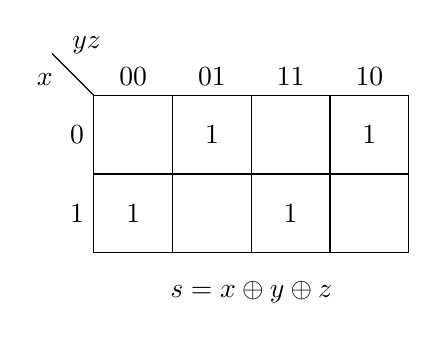
\begin{tikzpicture}
\pgfmathsetmacro{\kxstep}{1}
\pgfmathsetmacro{\kystep}{1}
\pgfmathsetmacro{\kpin}{0.75}
\pgfmathsetmacro{\kmv}{0.15}
\pgfmathsetmacro{\kmva}{0.10}
\draw[xstep=\kxstep,ystep=\kystep](0,0) grid (4*\kxstep,-2*\kystep);
\draw(0,0)--++(135:\kpin)node[pos=0.75,above right]{$yz$}node[pos=0.75,below left]{$x$};
\foreach \kx/\xlb in {0/{00},1/{01},2/{11},3/{10}}{\draw(\kx*\kxstep+\kxstep/2,0)node[above]{$\xlb$};}
\foreach \ky/\ylb in {0/{0},1/{1}}{\draw(0,-\ky*\kystep-\kystep/2)node[left]{$\ylb$};}
\foreach \kx/\xlb in {1/1,3/{1}}{\draw(\kx*\kxstep+\kxstep/2,-\kystep/2)node[]{$\xlb$};}
\foreach \kx/\xlb in {0/1,2/1}{\draw(\kx*\kxstep+\kxstep/2,-1.5*\kystep)node[]{$\xlb$};}
%\foreach \kx/\xlb in {0/{1},1/1}{\draw(\kx*\kxstep+\kxstep/2,-2.5*\kystep)node[]{$\xlb$};}
%\foreach \kx/\xlb in {0/1,1/1,2/d}{\draw(\kx*\kxstep+\kxstep/2,-3.5*\kystep)node[]{$\xlb$};}
%\draw[gray,dashed] ($(2*\kxstep,-0*\kystep)+(\kmv,-\kmv)$) rectangle ($(3*\kxstep,-2*\kystep)+(-\kmv,\kmv)$);
%\draw[gray,dashed] ($(1*\kxstep,-1*\kystep)+(\kmva,-\kmva)$) rectangle ($(3*\kxstep,-2*\kystep)+(-\kmva,\kmva)$);
%\draw[gray,dashed] ($(2*\kxstep,-1*\kystep)+(-\kmv,\kmv)$) rectangle ($(4*\kxstep,-2*\kystep)+(-\kmv,-\kmv)$);
%\draw[gray,dashed] ($(0,-3*\kystep)+(-\kmv,-\kmv)$)--++(1*\kxstep,0)--++(0,-\kystep-\kmv);
%\draw[gray,dashed] ($(3*\kxstep,-0*\kystep)+(\kmv,\kmv)$)--++(0,-1*\kystep)--++(\kxstep+\kmv,0);
%\draw[gray,dashed] ($(3*\kxstep,-4*\kystep)+(\kmv,-\kmv)$)--++(0,1*\kystep)--++(\kxstep+\kmv,0);
%\draw(4*\kxstep-\kmv,-0.5*\kystep) to [out=0,in=180]++(0.5,-0.25)node[right]{$\overline{w}\,\overline{x}$};
%\draw(1.5*\kxstep-\kmv,-4*\kystep+\kmv) to [out=-90,in=180]++(0.5,-0.5)node[right]{$w\overline{y}$};
\draw(2*\kxstep,-2*\kystep-0.5)node[]{$s=x\oplus y\oplus z$};
\end{tikzpicture}
\end{subfigure}
\caption{مکمل جمع کار}
\label{شکل_ترکیبی_مکمل_جمع}
\end{figure}

کارناف نقشہ استعمال کیے بغیر جدول \حوالہ{جدول_ترکیبی_مکمل_جمع_کار} سے ان تفاعلات کی مساوات، مجموعہ ارکان ضرب کے روپ میں لکھتے ہیں۔
\begin{gather}
\begin{aligned}\label{مساوات_ترکیبی_مکمل_جمع_کار_پہلا}
c&=\overline{x}yz+x\overline{y}z+xy\overline{z}+xyz\\
s&=\overline{x}\,\overline{y}z+\overline{x}y\overline{z}+x\overline{y}\,\overline{z}+xyz
\end{aligned}
\end{gather}
انہیں شکل \حوالہ{شکل_ترکیبی_مکمل_جمع_کار_پہلا} میں عملی جامہ پہنایا گیا ہے۔
%
\begin{figure}
\centering
\begin{subfigure}{0.45\textwidth}
\centering
\begin{tikzpicture}
\pgfmathsetmacro{\kxsep}{2};
\pgfmathsetmacro{\kysep}{1.5};
\pgfmathsetmacro{\kpin}{0.25};
\draw(0,0)node[and port ,scale=1, number inputs=3](u1){};
\draw(0,-1*\kysep)node[and port ,scale=1, number inputs=3](u2){};
\draw(0,-2*\kysep)node[and port ,scale=1, number inputs=3](u3){};
\draw(0,-3*\kysep)node[and port ,scale=1, number inputs=3](u4){};
 \draw(\kxsep,-1.5*\kysep)node[or port ,scale=1, number inputs=4](u5){};
 \draw(u1.out)-|(u5.in 1) (u4.out)-|(u5.in 4) (u5.in 2)--++(-\kpin,0)-|(u2.out) (u5.in 3)--++(-\kpin,0)-|(u3.out);
\draw[](u1.in 1)node[left]{$\overline{x}$} (u1.in 2)node[left]{$\overline{y}$} (u1.in 3)node[left]{$z$};
\draw[](u2.in 1)node[left]{$\overline{x}$} (u2.in 2)node[left]{$y$} (u2.in 3)node[left]{$\overline{z}$};
\draw[](u3.in 1)node[left]{$x$} (u3.in 2)node[left]{$\overline{y}$} (u3.in 3)node[left]{$\overline{z}$};
\draw[](u4.in 1)node[left]{$x$} (u4.in 2)node[left]{$y$} (u4.in 3)node[left]{$z$};
 \draw(u5.out)node[right]{$s$};
\end{tikzpicture}
\end{subfigure}\hfill
\begin{subfigure}{0.45\textwidth}
\centering
\begin{tikzpicture}
\pgfmathsetmacro{\kxsep}{2};
\pgfmathsetmacro{\kysep}{1.5};
\pgfmathsetmacro{\kpin}{0.25};
\draw(0,0)node[and port ,scale=1, number inputs=3](u1){};
\draw(0,-1*\kysep)node[and port ,scale=1, number inputs=3](u2){};
\draw(0,-2*\kysep)node[and port ,scale=1, number inputs=3](u3){};
\draw(0,-3*\kysep)node[and port ,scale=1, number inputs=3](u4){};
 \draw(\kxsep,-1.5*\kysep)node[or port ,scale=1, number inputs=4](u5){};
 \draw(u1.out)-|(u5.in 1) (u4.out)-|(u5.in 4) (u5.in 2)--++(-\kpin,0)-|(u2.out) (u5.in 3)--++(-\kpin,0)-|(u3.out);
\draw[](u1.in 1)node[left]{$\overline{x}$} (u1.in 2)node[left]{$y$} (u1.in 3)node[left]{$z$};
\draw[](u2.in 1)node[left]{$x$} (u2.in 2)node[left]{$\overline{y}$} (u2.in 3)node[left]{$z$};
\draw[](u3.in 1)node[left]{$x$} (u3.in 2)node[left]{$y$} (u3.in 3)node[left]{$\overline{z}$};
\draw[](u4.in 1)node[left]{$x$} (u4.in 2)node[left]{$y$} (u4.in 3)node[left]{$z$};
 \draw(u5.out)node[right]{$c$};
\end{tikzpicture}
\end{subfigure}
\caption{مکمل جمع کار (مساوات \حوالہ{مساوات_ترکیبی_مکمل_جمع_کار_پہلا})}
\label{شکل_ترکیبی_مکمل_جمع_کار_پہلا}
\end{figure}

درج بالا پہلی مساوات کے درمیانے دو اجزاء کا مجموعہ \عددی{x(\overline{y}z+y\overline{z})} جبکہ باقی اجزاء کا \عددی{(\overline{x}+x)yz} ہے، لہٰذا \عددی{c} کے لئے درج ذیل لکھا جا سکتا ہے۔
\begin{align*}
c&=(\overline{x}+x)yz+x(\overline{y}z+y\overline{z})\\
&=yz+x(y\oplus z)
\end{align*}
اس کو مساوات \حوالہ{مساوات_ترکیبی_مکمل_جمع_کار_کارناف} میں پیش \عددی{s} کے ساتھ اکٹھا لکھتے ہیں۔
\begin{gather}
\begin{aligned}\label{مساوات_ترکیبی_مکمل_جمع_کار_دوسرا}
c&=yz+x(y\oplus z)\\
s&=x\oplus y \oplus z
\end{aligned}
\begin{cases}
\begin{minipage}{0.2\textwidth}
مکمل جمع کار کی\\
بہتر مساوات
\end{minipage}
\end{cases}
\end{gather}
ان تفاعلات کو شکل \حوالہ{شکل_ترکیبی_مکمل_جمع_کار_دوسرا} میں پیش کیا گیا ہے، جو شکل \حوالہ{شکل_ترکیبی_مکمل_جمع_کار_پہلا} سے بہتر (چھوٹا)ہے۔
\begin{figure}
\centering
\begin{tikzpicture}
\pgfmathsetmacro{\kxsep}{2};
\pgfmathsetmacro{\kysep}{1.5};
\pgfmathsetmacro{\kpin}{1};
\draw(0,0)node[xor port ,scale=1, number inputs=2](u1){};
\draw(0,-1*\kysep)node[and port ,scale=1, number inputs=2](u2){};
\draw(2*\kxsep,0.5*\kysep)node[xor port ,scale=1, number inputs=2](u3){};
\draw(2*\kxsep,-0.5*\kysep)node[and port ,scale=1, number inputs=2](u4){};
 %\draw(3*\kxsep,-0.75*\kysep-0.1)node[or port ,scale=1, number inputs=2](u5){};
 \draw(u1.in 1)--++(-\kpin,0)coordinate(kla)coordinate[pos=0.4](kua)node[left]{$y$};
\draw(u1.in 2)--++(-\kpin,0)coordinate(klb)coordinate[pos=0.6](kuaa)node[left]{$z$};
\draw(kua)|-(u2.in 1) (kuaa)|-(u2.in 2); 
\draw(u3.in 1)--($(kla)!(u3.in 1)!(klb)$)coordinate(kll)node[left]{$x$};
\draw(u1.out)-|(u3.in 2);
\draw(u3.in 2)-|(u4.in 1);
\draw(u4.in 2)--++(-\kpin,0)coordinate(kcc)--($(u3.in 1)!(kcc)!(kll)$);
\draw(u2.out)--++(2.25*\kxsep,0)node[or port, scale=1,number inputs=2, anchor=in 2](u5){};
\draw(u4.out)-|(u5.in 1);
\draw(u5.out)node[right]{$c$};
\path(u5.out)--++(0,\kpin)coordinate(krr);
\draw(u3.out)--($(u5.out)!(u3.out)!(krr)$)node[right]{$s$};
\end{tikzpicture}
\caption{مکمل جمع کار کا بہتر دور (مساوات \حوالہ{مساوات_ترکیبی_مکمل_جمع_کار_دوسرا})}
\label{شکل_ترکیبی_مکمل_جمع_کار_دوسرا}
\end{figure}


مساوات \حوالہ{مساوات_ترکیبی_مکمل_جمع_کار_دوسرا} میں دیے \عددی{s} سے ارکان ضرب کا مجموعہ حاصل کرتے ہیں۔
\begin{align*}
s&=x\oplus (y\oplus z)\\
&=x\oplus (y\overline{z}+\overline{y}z)\\
&=x(\overline{y\overline{z}+\overline{y}z})+\overline{x}(y\overline{z}+\overline{y}z)\\
&=x(\overline{y\overline{z}})(\overline{\overline{y}z})+\overline{x}(y\overline{z}+\overline{y}z)\\
&=x(\overline{y}+z)(y+\overline{z})+\overline{x}(y\overline{z}+\overline{y}z)\\
&=x(yz+\overline{y}\,\overline{z})+\overline{x}(y\overline{z}+\overline{y}z)\\
&=xyz+x\overline{y}\,\overline{z}+\overline{x}y\overline{z}+\overline{x}\,\overline{y}z
\end{align*}
شکل \حوالہ{شکل_ترکیبی_مکمل_جمع_کار_دوسرا} \اصطلاح{ مکمل جمع کار}\فرہنگ{جمع کار!مکمل}\حاشیہب{full adder}\فرہنگ{adder!full} کہلاتا ہے ، لہٰذا شکل \حوالہ{شکل_ترکیبی_جمع_دو_بٹ} کو \اصطلاح{نصف جمع کار}\فرہنگ{جمع کار!نصف}\حاشیہب{half adder}\فرہنگ{adder!half} کہیں گے۔

جدول \حوالہ{جدول_ترکیبی_مکمل_جمع_کار} میں \عددی{y} اور \عددی{z} ثنائی ہندسوں کے ساتھ گزشتہ قدم کا حاصل \عددی{x} جمع کیا گیا۔ شکل \حوالہ{شکل_ترکیبی_مکمل_جمع_کار_ڈبہ} میں نصف جمع کار اور مکمل جمع کار کی علامت پیش ہیں۔ مکمل جمع کار میں گزشتہ قدم سے \اصطلاح{داخلی حاصل}\فرہنگ{حاصل!داخلی}\حاشیہب{carry in}\فرہنگ{carry!in} کو \عددی{c_{\text{د}}} جبکہ اس قدم کے \اصطلاح{خارجی حاصل}\فرہنگ{حاصل!خارجی}\حاشیہب{carry out}\فرہنگ{carry!out} کو \عددی{c_{\text{خ}}}سے ظاہر کیا گیا۔

\begin{figure}
\centering
\begin{tikzpicture}[
 fulladder/.style={draw, minimum height=1.5cm, minimum width=3cm,thick,
 label={[anchor=west]left:$c_\text{خ}$},
 label={[anchor=south]below:$s$},
 label={[anchor=east]right:$c_\text{د}$},
 label={[anchor=north]65:$z\vphantom{y}$},
 label={[anchor=north]115:$y\vphantom{z}$},
 },
 halfadder/.style={draw, minimum height=1.5cm, minimum width=3cm,thick,
 label={[anchor=west]left:$c$},
 label={[anchor=south]below:$s$},
 label={[anchor=north]65:$z\vphantom{y}$},
 label={[anchor=north]115:$y\vphantom{z}$},
 }]
\pgfmathsetmacro{\kpin}{0.5}
\node[fulladder] (a) {\text{\RL{مکمل جمع کار}}};
\draw[stealth-] (a.115) --++(90:\kpin) node [above] {};
\draw[stealth-] (a.65) --++(90:\kpin) node [above] {};
\draw[stealth-] (a.east) --++(\kpin,0) node [right] {};
\draw[-stealth] (a.west) --++(-\kpin,0) node [left] {};
\draw[-stealth] (a.south) --++(0,-\kpin) node [left] {};
 \node[halfadder, right=3cm of a] (b) {\text{\RL{نصف جمع کار}}};
\draw[stealth-] (b.115) --++(90:\kpin) node [above] {};
\draw[stealth-] (b.65) --++(90:\kpin) node [above] {};
\draw[-stealth] (b.west) --++(-\kpin,0) node [left] {};
\draw[-stealth] (b.south) --++(0,-\kpin) node [left] {};
\end{tikzpicture}
\caption{نصف جمع کار اور مکمل جمع کار کی علامتیں۔}
\label{شکل_ترکیبی_مکمل_جمع_کار_ڈبہ}
\end{figure}


آئیں \عددی{y=111_2} اور \عددی{z=11_2} کا مجموعہ مکمل جمع کار کی مدد سے حاصل کریں۔سب سے پہلے دونوں اعداد کو تین ثنائی ہندسوں میں لکھیں ، لہٰذا \عددی{z=011_2} ہو گا۔شکل \حوالہ{شکل_ترکیبی_تین_درجہ_جمع_کار} میں مطلوبہ تین درجی، تین بِٹ جمع کار پیش کیا گیا ہے، جہاں مکمل جمع کار کو مختصراً \قول{جمع کار} کہا گیا ہے ۔ ثنائی عدد \عددی{y=111=y_2y_1y_0} اور \عددی{z=011=z_2z_1z_0} ہیں۔یوں کم رتبی بِٹ کے مکمل جمع کار کو دونوں اعداد کے کم رتبی ہندسے، \عددی{y_0=1} اور \عددی{z_0=1}، فراہم کیے جائیں گے، اور ساتھ ہی چونکہ پہلے قدم میں کوئی \قول{داخلی حاصل} نہیں ہو گا لہٰذا داخلی حاصل \عددی{c_0=0} فراہم کیا جائے گا۔ اگلے قدم میں جمع کار کو \عددی{y_1=1} اور \عددی{z=1} کے ساتھ پہلے قدم کا حاصل \عددی{c_1} بطور داخلی حاصل، فراہم کیا جائے گا، جبکہ آخری جمع کار کو \عددی{y_2=1} اور \عددی{z_2=0} کے ساتھ گزشتہ قدم کا حاصل \عددی{c_2} فراہم کیا جائے گا۔تین بِٹ جمع کار، ان اعداد کا مجموعہ \عددی{c_3s_2s_1s_0=1010_2} دے گا۔
\begin{align*}
\begin{split}
111\phantom{1\,}&\\
\phantom{1}111&\\
+\phantom{1}011&\\
\noalign{\smallskip}\hline\noalign{\smallskip}
1010&
\end{split}
\end{align*}
%
\begin{figure}
\centering
\begin{tikzpicture}[
 fulladder/.style={draw, minimum height=1.5cm, minimum width=2cm,thick,
 label={[anchor=west]left:$c_\text{خ}$},
 label={[anchor=south]below:$s$},
 label={[anchor=east]right:$c_\text{د}$},
 label={[anchor=north]65:$z\vphantom{y}$},
 label={[anchor=north]115:$y\vphantom{z}$},
 }]
\pgfmathsetmacro{\kpin}{0.5}
\node[fulladder] (u0) {\text{\RL{جمع کار}}};
\node[fulladder, left=1cm of u0] (u1) {\text{\RL{جمع کار}}};
\node[fulladder, left=1cm of u1] (u2) {\text{\RL{جمع کار}}};
%
\draw[stealth-] (u0.115) --++(90:\kpin) node[above]{$1$}node [above,yshift=1.5em] {$y_0$};
\draw[stealth-] (u0.65) --++(90:\kpin) node[above]{$1$}node [above,yshift=1.5em] {$z_0$};
\draw[stealth-] (u1.115) --++(90:\kpin) node[above]{$1$}node [above,yshift=1.5em] {$y_1$};
\draw[stealth-] (u1.65) --++(90:\kpin) node[above]{$1$}node [above,yshift=1.5em] {$z_1$};
\draw[stealth-] (u2.115) --++(90:\kpin) node[above]{$1$}node [above,yshift=1.5em] {$y_2$};
\draw[stealth-] (u2.65) --++(90:\kpin) node[above]{$0$}node [above,yshift=1.5em] {$z_2$};
\draw[stealth-] (u0.east) --++(\kpin,0) node [right] {0}node[right,yshift=-1em]{$c_0$};
\draw[-stealth] (u0.south) --++(0,-\kpin)coordinate(ka) node[below]{$0$}node [below,yshift=-1.5em] {$s_0$};
\draw[-stealth] (u1.south) --++(0,-\kpin)coordinate(kb) node[below]{$1$}node [below,yshift=-1.5em] {$s_1$};
\draw[-stealth] (u2.south) --++(0,-\kpin) node[below]{$0$}node [below,yshift=-1.5em] {$s_2$};
\draw[-stealth](u0)--(u1)node[pos=0.5,above]{$1$}node[pos=0.5,below]{$c_1$};
\draw[-stealth](u1)--(u2)node[pos=0.5,above]{$1$}node[pos=0.5,below]{$c_2$};
\draw[-stealth](u2.west)--++(-\kpin,0)coordinate(kc)--($(ka)!(kc)!(kb)$)node[below]{$1$}node[below,yshift=-1.5em]{$c_3$};
\draw(u0.south)node[yshift=-1.75cm]{\text{\RL{درجہ صفر}}};
\draw(u1.south)node[yshift=-1.75cm]{\text{\RL{درجہ ایک}}};
\draw(u2.south)node[yshift=-1.75cm]{\text{\RL{درجہ دو}}};
\end{tikzpicture}
\caption{تین درجی، تین بِٹ جمع کار}
\label{شکل_ترکیبی_تین_درجہ_جمع_کار}
\end{figure}

شکل \حوالہ{شکل_ترکیبی_تین_درجہ_جمع_کار} میں چونکہ درجہ صفر کا داخلی حاصل ہمیشہ \عددی{0} ہو گا لہٰذا یہاں مکمل جمع کار کی بجائے نصف جمع کار بھی استعمال کیا جا سکتا تھا۔ ایسا کرتے ہوئے \عددی{c_0} فراہم کرنے کی ضرورت نہیں ہو گی۔

 زیادہ بِٹ اعداد کے مجموعہ کے لئے شکل \حوالہ{شکل_ترکیبی_تین_درجہ_جمع_کار} میں بائیں جانب مزید مکمل جمع کار کا اضافہ کیا جائے گا۔ یوں \عددی{8} بِٹ (یعنی ایک بائٹ) اعداد کا مجموعہ آٹھ درجی جمع کار دے گا، جو \عددی{8} مکمل جمع کار پر مشتمل ہو گا، جبکہ \عددی{64} بِٹ اعداد کے مجموعہ کے لئے \عددی{64} مکمل جمع کار پر مشتمل \عددی{64} بِٹ جمع کار درکار ہو گا۔


\ابتدا{مشق}
مخلوط دور 74283 چار بِٹ مکمل جمع کار ہے (صفحہ \حوالہصفحہ{بوولین_مخلوط_ادوار_سلسلہ} پر مخلوط ادوار کے سلسلہ \عددی{74xxx} کے بارے میں دوبارہ پڑھیں)۔اس کے معلوماتی صفحات انٹرنیٹ\حاشیہد{انٹرنیٹ میں \تحریر{74283 datasheet} تلاش کریں۔} سے حاصل کریں۔ اس مخلوط دور کو استعمال کرتے ہوئے \عددی{8} بٹ کے دو ثنائی اعداد جمع کریں۔
\انتہا{مشق}

\جزوحصہ{منفی کار}
 ثنائی اعداد کو کمپیوٹر دو کے تکملہ کی مدد سے منفی کرتا ہے۔دو کا تکملہ استعمال کرتے ہوئے ثنائی اعداد منفی کرنے کے عمل پر دوبارہ نظر ڈالتے ہیں۔یاد رہے، بلند تر رتبی بِٹ کی جمع سے پیدا، آخری حاصل ضائع کیا جاتا ہے،جبکہ اس کی غیر موجودگی میں نتیجے کا دو کا تکملہ لیا جاتا ہے۔

 ثنائی عدد کے اساس منفی ایک تکملہ (یا متمم) کے ساتھ \عددی{1} جمع کرنے سے عدد کا اساسی تکملہ حاصل ہو گا۔ عدد کا متمم حاصل کرنے کی خاطر عدد کے ہر بِٹ کا متمم لیا جاتا ہے۔بِٹ کا متمم بذریعہ نفی گیٹ لیا جا سکتا ہے۔
	
تین بِٹ ثنائی اعداد \عددی{y} اور \عددی{z} سے \عددی{(y-z)} حاصل کرنے کے لئے \عددی{z} کے متمم کے ساتھ \عددی{1} اور \عددی{y} جمع کرنا ہو گا۔
شکل \حوالہ{شکل_ترکیبی_تین_درجہ_منفی_کار} میں اس عمل کو عملی جامہ پہنایا گیا ہے، جہاں نفی گیٹ استعمال کر کے \عددی{z} کا متمم (یا ایک کا تکملہ) حاصل کیا گیا، اور ساتھ \عددی{1} جمع کرنے کی خاطر درجہ صفر کو داخلی حاصل \عددی{1} فراہم کیا گیا۔

\begin{figure}
\centering
\begin{tikzpicture}[
 fulladder/.style={draw, minimum height=1.5cm, minimum width=2.25cm,thick,
 label={[anchor=west]left:$c_\text{خ}$},
 label={[anchor=south]below:$s$},
 label={[anchor=east]right:$c_\text{د}$},
 label={[anchor=north]65:$z\vphantom{y}$},
 label={[anchor=north]115:$y\vphantom{z}$},
 }]
\pgfmathsetmacro{\kpin}{0.5}
\pgfmathsetmacro{\kpina}{0.15}
\node[fulladder] (u0) {\text{\RL{جمع کار}}};
\node[fulladder, left=1cm of u0] (u1) {\text{\RL{جمع کار}}};
\node[fulladder, left=1cm of u1] (u2) {\text{\RL{جمع کار}}};
%
\draw[stealth-] (u0.65) --++(90:\kpina) coordinate(knota);
\draw (knota)node[not port,scale=0.8,rotate=-90,anchor=out](u4){} (u4.in)node[above]{$z_0$};
\draw[stealth-] (u1.65) --++(90:\kpina)coordinate(knotb);
\draw (knotb)node[not port,scale=0.8,rotate=-90,anchor=out](u5){} (u5.in)node[above]{$z_1$};
\draw[stealth-] (u2.65) --++(90:\kpina)coordinate(knotc);
\draw (knotc)node[not port,scale=0.8,rotate=-90,anchor=out](u6){} (u6.in)node[above]{$z_2$};
\draw[stealth-] (u0.115) --($(u4.in)!(u0.115)!(u5.in)$) node[above]{$y_0$};
\draw[stealth-] (u1.115) --($(u4.in)!(u1.115)!(u5.in)$) node[above]{$y_1$};
\draw[stealth-] (u2.115) --($(u4.in)!(u2.115)!(u5.in)$) node[above]{$y_2$};
\draw[stealth-] (u0.east) --++(\kpin,0) node [right] {1};
\draw[-stealth] (u0.south) --++(0,-\kpin)coordinate(ka) node[below]{$s_0$};
\draw[-stealth] (u1.south) --++(0,-\kpin)coordinate(kb) node[below]{$s_1$};
\draw[-stealth] (u2.south) --++(0,-\kpin) node[below]{$s_2$};
\draw[-stealth](u0)--(u1);
\draw[-stealth](u1)--(u2);
\draw[-stealth](u2.west)--++(-\kpin,0);
\end{tikzpicture}
\caption{تین درجی، تین بِٹ منفی کار}
\label{شکل_ترکیبی_تین_درجہ_منفی_کار}
\end{figure}

شکل \حوالہ{شکل_ترکیبی_تین_درجہ_جمع_کار} اور شکل \حوالہ{شکل_ترکیبی_تین_درجہ_منفی_کار} دونوں میں مکمل جمع کار استعمال ہوئے۔شکل \حوالہ{شکل_ترکیبی_تین_درجہ_جمع_کار} کے ساتھ نفی گیٹ منسلک کر کے اور داخلی حاصل \عددی{c_0} کو \عددی{0} کی بجائے \عددی{1} رکھنے سے شکل \حوالہ{شکل_ترکیبی_تین_درجہ_منفی_کار} حاصل ہو گا۔ جمع اور منفی اعمال ایک ہی دور سے بھی حاصل کیے جا سکتے ہیں۔ایسا دور جسے جمع و منفی کار کہتے ہیں شکل \حوالہ{شکل_ترکیبی_تین_درجہ_جمع_و_منفی_کار} میں پیش ہے۔
\begin{figure}
\centering
\begin{tikzpicture}[
 fulladder/.style={draw, minimum height=1.5cm, minimum width=2cm,thick,
 label={[anchor=west]left:$c_\text{خ}$},
 label={[anchor=south]below:$s$},
 label={[anchor=east]right:$c_\text{د}$},
 label={[anchor=north]65:$z\vphantom{y}$},
 label={[anchor=north]115:$y\vphantom{z}$},
 }]
\pgfmathsetmacro{\kpin}{0.5}
\pgfmathsetmacro{\kpina}{0.25}
\node[fulladder] (u0) {\text{\RL{جمع کار}}};
\node[fulladder, left=1cm of u0] (u1) {\text{\RL{جمع کار}}};
\node[fulladder, left=1cm of u1] (u2) {\text{\RL{جمع کار}}};
%
\draw[stealth-] (u0.65) --++(90:\kpina) coordinate(knota);
\draw (knota)node[xor port,scale=0.75,number inputs=2,rotate=-90,anchor=out](u4){}
 (u4.in 1)--++(0,\kpin)coordinate(kaa)node[above]{$z_0$};
\draw[stealth-] (u1.65) --++(90:\kpina)coordinate(knotb);
\draw (knotb)node[xor port,scale=0.75,number inputs=2,rotate=-90,anchor=out](u5){}
 (u5.in 1)--++(0,\kpin)coordinate(kbb)node[above]{$z_1$};
\draw[stealth-] (u2.65) --++(90:\kpina)coordinate(knotc);
\draw (knotc)node[xor port,scale=0.75,number inputs=2,rotate=-90,anchor=out](u6){} 
(u6.in 1)--++(0,\kpin)node[above]{$z_2$};
\draw[stealth-] (u0.115) --($(kaa)!(u0.115)!(kbb)$) node[above]{$y_0$};
\draw[stealth-] (u1.115) --($(kaa)!(u1.115)!(kbb)$) node[above]{$y_1$};
\draw[stealth-] (u2.115) --($(kaa)!(u2.115)!(kbb)$) node[above]{$y_2$};
\draw[stealth-] (u0.east) --++(\kpin,0)node[below]{$c_0$}coordinate(kff)--($(u4.in 2)!(kff)!(u5.in 2)$)--(u4.in 2);
\draw[-stealth] (u0.south) --++(0,-\kpin)coordinate(ka) node[below]{$s_0$};
\draw[-stealth] (u1.south) --++(0,-\kpin)coordinate(kb) node[below]{$s_1$};
\draw[-stealth] (u2.south) --++(0,-\kpin) node[below]{$s_2$};
\draw[-stealth](u0)--(u1)node[pos=0.5,below]{$c_1$};
\draw[-stealth](u1)--(u2)node[pos=0.5,below]{$c_2$};
\draw[-stealth](u2.west)--++(-\kpin,0)coordinate(kcc)node[below]{$c_3$};
\path(kcc)--++(0,\kpin)coordinate(kdd);
\draw(u4.in 2)--(u5.in 2)--(u6.in 2)--($(kcc)!(u6.in 2)!(kdd)$)node[left]{\RL{{$\overline{\text{جمع}}$}/منفی}};
\end{tikzpicture}
\caption{تین بِٹ جمع و منفی کار}
\label{شکل_ترکیبی_تین_درجہ_جمع_و_منفی_کار}
\end{figure}

اس شکل میں بلا شرکت جمع گیٹ استعمال کیا گیا، اور قابو اشارہ {{$\overline{\text{جمع}}$}/منفی} کا اضافہ کیا گیا۔اس قابو اشارہ کی کارکردگی پر غور کرتے ہیں۔جب {{$\overline{\text{جمع}}$}/منفی} اشارہ پست \عددی{(0)}ہو بلا شرکت جمع گیٹ عدد \عددی{z} جوں کا توں مکمل جمع کار تک پہنچائے گا، اور ساتھ ہی \عددی{c_0=0}ہو گا؛لہٰذا یہ دور تین بِٹ جمع کار کی حیثیت سے کام کرے گا۔

اس کے برعکس،{{$\overline{\text{جمع}}$}/منفی} اشارہ بلند \عددی{(1)}ہو بلا شرکت جمع گیٹ عدد \عددی{z} کا متمم \عددی{\overline{z}} مکمل جمع کار تک پہنچائے گا، اور ساتھ ہی \عددی{c_0=1}ہو گا؛لہٰذا یہ دور تین بِٹ منفی کار کی حیثیت سے کام کرے گا۔
	
قابو اشارہ کے نام میں \قول{منفی} اور \قول{\عددیء{\overline{جمع}}} لکھ کر یہ واضح کی گیا ہے کہ اشارہ بلند ہونے کی صورت میں منفی کار اور پست ہونے کی صورت میں جمع کار حاصل ہو گا۔

	
آٹھ بِٹ جمع و منفی کار کو ایک بائٹ جمع و منفی کار کہتے ہیں۔ شکل \حوالہ{شکل_ترکیبی_دو_بائٹ_جمع_و_منفی_کار} میں ایک بائٹ اور دو بائٹ جمع و منفی کار دکھائے گئے ہیں۔اس کے بائیں جانب مزید درجات جوڑ کر متعدد بائٹ کا دور بنایا جا سکتا ہے۔ یہاں \عددی{Y_0} پہلے بائٹ (یعنی بِٹ \عددی{y_0} تا \عددی{y_7}) کو، \عددی{Y_1} اگلے بائٹ (یعنی بِٹ \عددی{y_8} تا \عددی{y_{14}}) کو ظاہر کرتا ہے، جبکہ \عددی{C_2} سے مراد دوسرے بائٹ کی جمع کا خارجی حاصل ہے۔

\begin{figure}
\centering
\begin{subfigure}{1\textwidth}
\centering
\begin{tikzpicture}
\pgfmathsetmacro{\kul}{0.75}
\pgfmathsetmacro{\kpsep}{0.15}
\pgfmathsetmacro{\kum}{0.75}
\pgfmathsetmacro{\kur}{0.5}
\pgfmathsetmacro{\kus}{\kul+7*\kpsep+\kum}
\pgfmathsetmacro{\kll}{\kus}
\pgfmathsetmacro{\kxdim}{\kul+14*\kpsep+\kum+\kur}
\pgfmathsetmacro{\kydim}{1.25}
\pgfmathsetmacro{\kpin}{0.5}
\pgfmathsetmacro{\kpina}{1}
\pgfmathsetmacro{\kvspace}{6}
\pgfmathsetmacro{\khspace}{\kxdim+0.75}
\pgfmathsetmacro{\kvcon}{1.25}
\draw[thick](0,0) rectangle ++(\kxdim,\kydim)node[pos=0.5]{\text{\RL{آٹھ بِٹ جمع و منفی کار}}};
\foreach \x in {0,1,2,3,4,5,6,7}{\draw[stealth-](\kul+\x*\kpsep,\kydim)--++(0,\kpin);}
\foreach \x in {0,1,2,3,4,5,6,7}{\draw[stealth-](\kus+\x*\kpsep,\kydim)--++(0,\kpin);}
\foreach \x in {0,1,2,3,4,5,6,7}{\draw[-stealth](\kll+\x*\kpsep,0)--++(0,-\kpin);}
\draw (\kul+3.5*\kpsep,\kydim+0.75)node[]{$Y$};
\draw (\kus+3.5*\kpsep,\kydim+0.75)node[]{$Z$};
\draw (\kll+3.5*\kpsep,-0.75)node[]{$S$};
\draw[-stealth](-\kpin,\kydim+\kvcon)node[left]{\RL{{$\overline{\text{جمع}}$}/منفی}}
--++(1.5*\kpin,0)coordinate(ucon)--++(0,-\kvcon);
\draw[-stealth](ucon)--++(\kxdim,0)--++(0,-\kydim/2-\kvcon)node[right]{$c_0$}--++(-0.5*\kpin,0);
\draw[-stealth](0,\kydim/2)--++(-\kpin,0)node[left]{$c_8$};
\end{tikzpicture}
\end{subfigure}
\begin{subfigure}{1\textwidth}
\centering
\begin{tikzpicture}
\pgfmathsetmacro{\kul}{0.75}
\pgfmathsetmacro{\kpsep}{0.15}
\pgfmathsetmacro{\kum}{0.75}
\pgfmathsetmacro{\kur}{0.5}
\pgfmathsetmacro{\kus}{\kul+7*\kpsep+\kum}
\pgfmathsetmacro{\kll}{\kus}
\pgfmathsetmacro{\kxdim}{\kul+14*\kpsep+\kum+\kur}
\pgfmathsetmacro{\kydim}{1.25}
\pgfmathsetmacro{\kpin}{0.5}
\pgfmathsetmacro{\kpina}{1}
\pgfmathsetmacro{\kvspace}{6}
\pgfmathsetmacro{\khspace}{\kxdim+0.75}
\pgfmathsetmacro{\kvcon}{1.25}
\draw[thick](0,0) rectangle ++(\kxdim,\kydim)node[pos=0.5]{\text{\RL{آٹھ بِٹ جمع و منفی کار}}};
\foreach \x in {0,1,2,3,4,5,6,7}{\draw[stealth-](\kul+\x*\kpsep,\kydim)--++(0,\kpin);}
\foreach \x in {0,1,2,3,4,5,6,7}{\draw[stealth-](\kus+\x*\kpsep,\kydim)--++(0,\kpin);}
\foreach \x in {0,1,2,3,4,5,6,7}{\draw[-stealth](\kll+\x*\kpsep,0)--++(0,-\kpin);}
\draw (\kul+3.5*\kpsep,\kydim+0.75)node[]{$Y_1$};
\draw (\kus+3.5*\kpsep,\kydim+0.75)node[]{$Z_1$};
\draw (\kll+3.5*\kpsep,-0.75)node[]{$S_1$};
%
\draw[thick](\khspace,0) rectangle ++(\kxdim,\kydim)node[pos=0.5]{\text{\RL{آٹھ بِٹ جمع و منفی کار}}};
\foreach \x in {0,1,2,3,4,5,6,7}{\draw[stealth-](\khspace+\kul+\x*\kpsep,\kydim)--++(0,\kpin);}
\foreach \x in {0,1,2,3,4,5,6,7}{\draw[stealth-](\khspace+\kus+\x*\kpsep,\kydim)--++(0,\kpin);}
\foreach \x in {0,1,2,3,4,5,6,7}{\draw[-stealth](\khspace+\kll+\x*\kpsep,0)--++(0,-\kpin);}
\draw (\khspace+\kul+3.5*\kpsep,\kydim+0.75)node[]{$Y_0$};
\draw (\khspace+\kus+3.5*\kpsep,\kydim+0.75)node[]{$Z_0$};
\draw (\khspace+\kll+3.5*\kpsep,-0.75)node[]{$S_0$};
\draw[-stealth](-\kpin,\kydim+\kvcon)node[left]{\RL{{$\overline{\text{جمع}}$}/منفی}}
--++(1.5*\kpin,0)coordinate(kcon)--++(0,-\kvcon);
\draw[-stealth](kcon)--++(\khspace,0)coordinate(kconr)--++(0,-\kvcon);
\draw(kconr)--++(\kxdim+0.5*\kpin,0)--++(0,-\kydim/2-\kvcon)node[below]{$C_0$}--++(-\kpin,0);
\draw[-stealth](0,\kydim/2)--++(-\kpin,0)node[below]{$C_2$};
\draw[stealth-](\kxdim,\kydim/2)--(\khspace,\kydim/2)node[pos=0.5,below]{$C_1$};
\end{tikzpicture}
\end{subfigure}
\caption{ایک اور دو بائٹ جمع و منفی کار}
\label{شکل_ترکیبی_دو_بائٹ_جمع_و_منفی_کار}
\end{figure}


\جزوحصہ{ اعشاری جمع کار}
جیسا پہلے ذکر ہوا، اعشاری اعداد کو \اصطلاح{ثنائی مرموز اعشاریہ}\فرہنگ{ثنائی مرموز اعشاریہ}\حاشیہب{binary coded decimal (BCD)}\فرہنگ{binary coded decimal (BCD)} سے ظاہر کیا جاتا ہے۔ ایسا مکمل جمع کار بناتے ہیں جو دو اعشاری ہندسوں \عددی{M}، \عددی{N} اور داخلی حاصل \عددی{c_d} کو جمع کرتا ہو۔چونکہ اعشاری ہندسے \عددی{0} تا \عددی{9} ، جبکہ داخلی حاصل \عددی{0} یا \عددی{1} ہو سکتا ہے، لہٰذا اس جمع کار کے جواب \عددی{(M+N+c_d)} کی قیمت \عددی{(0+0+0=0)} تا \عددی{(9+9+1=19)} ہو گی، جنہیں اعشاری، ثنائی مرموز اعشاریہ اور ثنائی روپ میں جدول \حوالہ{جدول_ترکیبی_ثنائی_مرموز_اعشاریہ} میں پیش کیا گیا ہے۔

\begin{table}
\caption{اعشاری جمع کار کے مطلوبہ جواب}
\label{جدول_ترکیبی_ثنائی_مرموز_اعشاریہ}
\centering
\begin{otherlanguage}{english}
\begin{tabular}{CCCCC|CCCCC|R}
\toprule
\multicolumn{5}{c|}{\text{\RL{ثنائی}}}&\multicolumn{5}{c|}{\text{\RL{ثنائی مرموز اعشاریہ}}}&\text{\RL{اعشاری}}\\
b_4&b_3&b_2&b_1&b_0&c&d_3&d_2&d_1&d_0&\\
\midrule
0&0&0&0&0&0&0&0&0&0&0\\
0&0&0&0&1&0&0&0&0&1&1\\
0&0&0&1&0&0&0&0&1&0&2\\
0&0&0&1&1&0&0&0&1&1&3\\
0&0&1&0&0&0&0&1&0&0&4\\
0&0&1&0&1&0&0&1&0&1&5\\
0&0&1&1&0&0&0&1&1&0&6\\
0&0&1&1&1&0&0&1&1&1&7\\
0&1&0&0&0&0&1&0&0&0&8\\
0&1&0&0&1&0&1&0&0&1&9\\
\midrule
0&1&0&1&0&1&0&0&0&0&10\\
0&1&0&1&1&1&0&0&0&1&11\\
0&1&1&0&0&1&0&0&1&0&12\\
0&1&1&0&1&1&0&0&1&1&13\\
0&1&1&1&0&1&0&1&0&0&14\\
0&1&1&1&1&1&0&1&0&1&15\\
1&0&0&0&0&1&0&1&1&0&16\\
1&0&0&0&1&1&0&1&1&1&17\\
1&0&0&1&0&1&1&0&0&0&18\\
1&0&0&1&1&1&1&0&0&1&19\\
\bottomrule
\end{tabular}
\end{otherlanguage}
\end{table}

 جدول میں، چار بِٹ ثنائی روپ میں خارجی حاصل کو \عددی{b_4} ، جبکہ ثنائی مرموز اعشاریہ میں خارجی حاصل کو \عددی{c} سے ظاہر کیا گیا ہے۔ان طریقوں میں \عددی{0} تا \عددی{9} جوابات ایک جیسے، جبکہ \عددی{10} تا \عددی{19} ایک دوسرے سے مختلف لکھے جاتے ہیں۔یوں اگر چار بِٹ ثنائی جمع کار استعمال ہو اور جواب \عددی{0} تا \عددی{9} ہو تب یہی جواب بطور ثنائی مرموز اعشاریہ جواب قابل قبول ہو گا، البتہ \عددی{9} سے بڑے ثنائی جواب کو ثنائی مرموز اعشاریہ جواب تسلیم نہیں کیا جا سکتا۔آئیں دیکھتے ہیں ایسی صورت میں کیا کیا جا سکتا ہے۔

یہاں ایک دلچسپ حقیقت پر غور کرتے ہیں۔ نا قابل قبول ثنائی جواب کے ساتھ \عددی{0110_2} ثنائی طور جمع کرنے سے درست ثنائی مرموز اعشاریہ جواب حاصل ہو گا۔مثلاً،\عددی{01010_2} کے ساتھ \عددی{0110_2} جمع کرنے سے \عددی{10000_2} حاصل ہو گا، جو ثنائی مرموز اعشاریہ میں درست جواب ہے۔ یوں \عددی{0} تا \عددی{9} ثنائی جوابات کو جوں کا توں، جبکہ ان سے بڑے جوابات کے ساتھ \عددی{0110_2} ثنائی طور جمع کر کے ثنائی مرموز اعشاریہ جواب حاصل کیے جا سکتے ہیں۔

	
جدول سے واضح ہے کہ جب ثنائی جمع کار کے جواب میں خارجی حاصل \عددی{b_4} بلند ہو، اس جواب کو ثنائی مرموز اعشاریہ جواب تسلیم نہیں کیا جا سکتا؛ اس کے علاوہ جب \عددی{b_3} کے ساتھ \عددی{b_2} یا \عددی{b_1} بھی بلند ہو تب بھی جواب کو ثنائی مرموز اعشاریہ تسلیم نہیں کیا جا سکتا۔ ان حقائق کو درج ذیل بوولین مساوات بیان کرتی ہے، جہاں ناقابل قبول جواب کی صورت میں \عددی{G} بلند ہو گا۔
 \begin{align}
 G=b_4+b_3b_2+b_3b_1
 \end{align}
اس حقیقت کو استعمال کرتے ہوئے ثنائی جمع کار کی مدد سے ثنائی مرموز اعشاریہ جمع کار کا حصول شکل \حوالہ{شکل_ترکیبی_اعشاری_جمع_کار} میں دکھایا گیا ہے۔
\begin{figure}
\centering
\begin{tikzpicture}
\pgfmathsetmacro{\kul}{0.5}
\pgfmathsetmacro{\kpsep}{0.40}
\pgfmathsetmacro{\kum}{0.75}
\pgfmathsetmacro{\kur}{0.5}
\pgfmathsetmacro{\kll}{1.5}
\pgfmathsetmacro{\kus}{\kul+3*\kpsep+\kum}
\pgfmathsetmacro{\kxdim}{\kul+6*\kpsep+\kum+\kur}
\pgfmathsetmacro{\kydim}{1.25}
\pgfmathsetmacro{\kpin}{0.5}
\pgfmathsetmacro{\kpina}{1}
\pgfmathsetmacro{\kvspace}{5}
\draw[thick](0,0) rectangle ++(\kxdim,\kydim)node[pos=0.5,yshift=0.5em]{\text{\RL{چار بِٹ ثنائی جمع کار}}};
\foreach \x in {0,1,2,3}{\draw[](\kul+\x*\kpsep,\kydim)--++(0,\kpin);}
\foreach \x in {0,1,2,3}{\draw[](\kus+\x*\kpsep,\kydim)--++(0,\kpin);}
\draw(\kxdim,\kydim/2)--++(\kpin,0)node[right]{$c_d$};
\draw (\kul+1.5*\kpsep,\kydim+0.75)node[]{$M$};
\draw (\kus+1.5*\kpsep,\kydim+0.75)node[]{$N$};
\draw[thick](0,-\kvspace) rectangle ++(\kxdim,\kydim)node[pos=0.5,yshift=0.5em]{\text{\RL{چار بِٹ ثنائی جمع کار}}};
\foreach \x/\d in {0/{d_3},1/{d_2},2/{d_1},3/{d_0}}{\draw[](\kus+\x*\kpsep,-\kvspace)--++(0,-\kpin)node[below]{$\d$};}
\foreach \x/\b in {0/{b_3},1/{b_2},2/{b_1},3/{b_0}}{\draw[](\kus+\x*\kpsep,-\kvspace+\kydim)--++(0,\kvspace-\kydim)node[above]{$\b$};}
\draw(\kxdim,-\kvspace+\kydim/2)--++(\kpin,0)node[right]{$0$};
\draw(0,-\kvspace+\kydim/2)--++(-\kpin,0)--++(0,-\kydim/2-\kpin)node[below]{$c$};
%
\draw(\kus-2*\kpsep,-0.50)node[and port, scale=1,number inputs=2,rotate=180,anchor=in 2](u1){};
\draw(\kus-2*\kpsep,-1.75)node[and port, scale=1,number inputs=2,rotate=180, anchor=in 2](u2){};
\draw(u1.out)++(-2,0)node[or port, scale=1,number inputs=3,rotate=180](u3){};
\draw(0,\kydim/2)node[above left]{$b_4$}-|(u3.in 3) (u1.out)--(u3.in 2) (u2.out)-|(u3.in 1);
\draw(u1.in 1)--++(2*\kpsep,0) (u1.in 2)--++(3*\kpsep,0) (u2.in 1)--++(2*\kpsep,0) (u2.in 2)--++(4*\kpsep,0);
%
\foreach \x in {0,3}{\draw[](\kul+\x*\kpsep,-\kvspace+\kydim)--++(0,\kpin);}
\foreach \x in {1,2}{\draw[](\kul+\x*\kpsep,-\kvspace+\kydim)--++(0,\kpina);}
\draw(\kul+3*\kpsep,-\kvspace+\kydim)++(0,\kpin)--++(-2,0)node[left]{$0$};
\draw(\kul+2*\kpsep,-\kvspace+\kydim)++(0,\kpina)--++(-2,0)-|(u3.out)node[above left]{$G$};
\end{tikzpicture}
\caption{ثنائی مرموز اعشاریہ روپ میں اعشاری جمع کار}
\label{شکل_ترکیبی_اعشاری_جمع_کار}
\end{figure}
 اگر \عددی{G} پست ہو تب نچلا جمع کار بالائی جمع کار کے جواب کے ساتھ \عددی{0} جمع کر کے اسی جواب کو خارج کرتا ہے، جبکہ \عددی{G} بلند ہونے کی صورت میں ساتھ \عددی{0110_2} جمع کر کے درست ثنائی مرموز اعشاریہ خارج کرتا ہے۔


\حصہ{ثنائی ضرب کار}
ثنائی ضرب بالکل اعشاری ضرب کی طرح کی جاتی ہے۔دو بِٹ ثنائی اعداد \عددی{y} اور \عددی{z} کو قلم و کاغذ کی طرز پر ضرب کرتے ہیں۔
\begin{align*}
\begin{array}{cccc}
&& z_1&z_0\\
&& y_1&y_0\\
\cline{3-4}
&& y_0z_1&y_0z_0\\
&y_1z_1&y_1z_0&\\
\cline{1-4}
m_3&m_2&m_1&m_0
\end{array}
\end{align*}
اس مساوات سے حاصل دو بِٹ ثنائی ضرب کار شکل \حوالہ{شکل_ترکیبی_دو_بٹ_ضرب_کار} میں پیش ہے۔زیادہ بِٹ کے ضرب کار بھی اسی طرح تشکیل دیے جاتے ہیں۔

 درج بالا قلم و کاغذ کی طرز پر ضرب میں کمتر بِٹ \عددی{m_0=y_0z_0} ہے جو شکل میں جمع گیٹ \عددی{u_4} دیتا ہے۔ اگلا بِٹ \عددی{m_1} ہے جو \عددی{y_0z_1} اور \عددی{y_1z_0} کو جمع کر کے حاصل ہو گا۔ جمع گیٹ \عددی{u_3} ہمیں \عددی{y_0z_1} جبکہ \عددی{u_2} ہمیں \عددی{y_1z_0} دیتا ہے، جنہیں دایاں نصف جمع کار \عددی{u_6} آپس میں جمع کر کے \عددی{m_1} اور حاصل (اگر موجود ہو) دیتا ہے۔ اس حاصل کو \عددی{y_1z_1} (جو گیٹ \عددی{u_1} سے ملتا ہے) کے ساتھ بایاں نصف جمع کار \عددی{u_5} ملا کر \عددی{m_2} اور حاصل \عددی{m_3} دیگا۔ 
\begin{figure}
\centering
\begin{tikzpicture}
\pgfmathsetmacro{\kul}{1}
\pgfmathsetmacro{\kpsep}{0.15}
\pgfmathsetmacro{\kum}{1.5}
\pgfmathsetmacro{\kur}{\kul}
\pgfmathsetmacro{\kus}{\kul+\kum}
\pgfmathsetmacro{\kll}{\kus}
\pgfmathsetmacro{\kxdim}{\kul+\kum+\kur}
\pgfmathsetmacro{\kydim}{1.25}
\pgfmathsetmacro{\kpin}{0.5}
\pgfmathsetmacro{\kpina}{1.5}
\pgfmathsetmacro{\kvspace}{6}
\pgfmathsetmacro{\khspace}{\kxdim+1.5}
\pgfmathsetmacro{\kcona}{3}
\pgfmathsetmacro{\kconb}{2.5}
\pgfmathsetmacro{\kconc}{2}
\draw[thick](0,0) rectangle ++(\kxdim,\kydim)node [pos=0.5,below]{$u_5$}node[pos=0.5,above]{\text{\RL{نصف جمع کار}}};
\draw[thick](\khspace,0) rectangle ++(\kxdim,\kydim)node [pos=0.5,below]{$u_6$}node[pos=0.5,above]{\text{\RL{نصف جمع کار}}};
\draw(\kul,\kydim)node[and port,scale=1,number inputs=2,rotate=-90,anchor=out](u1){\rotatebox{90}{$u_1$}};
\draw(\kul+\khspace,\kydim)node[and port,scale=1,number inputs=2,rotate=-90,anchor=out](u2){\rotatebox{90}{$u_2$}};
\draw(\kus+\khspace,\kydim)node[and port,scale=1,number inputs=2,rotate=-90,anchor=out](u3){\rotatebox{90}{$u_3$}};
\draw(\khspace+\kxdim+\kpin,\kydim)node[and port,scale=1,number inputs=2,rotate=-90,anchor=out](u4){\rotatebox{90}{$u_4$}};
\draw(-\kpin,\kydim+\kconb)node[left]{$y_1$}-|(u2.in 2);
\draw(\khspace+\kxdim+\kpina,\kydim+\kconb)node[right]{$z_0$}-|(u2.in 1);
\path(-\kpina,\kydim+\kconb)--++(\kpin,0)coordinate(aa);
\draw(u1.in 2)--($(-\kpina,\kydim+\kconb)!(u1.in 2)!(aa)$);
\draw(\khspace+\kxdim+\kpina,\kydim+\kconc)node[right]{$z_1$}-|(u1.in 1);
\path(\khspace+\kxdim+\kpina,\kydim+\kconc)--++(-\kpin,0)coordinate(bb);
\draw(u3.in 1)--($(\khspace+\kxdim+\kpina,\kydim+\kconc)!(u3.in 1)!(bb)$);
\path(\khspace+\kxdim+\kpina,\kydim+\kconb)--++(-\kpin,0)coordinate(cc);
\draw(u4.in 1)--($(\khspace+\kxdim+\kpina,\kydim+\kconb)!(u4.in 1)!(cc)$);
\draw(-\kpin,\kydim+\kcona)node[left]{$y_0$}-|(u4.in 2);
\path(-\kpin,\kydim+\kcona)--++(-\kpin,0)coordinate(dd);
\draw(u3.in 2)--($(-\kpin,\kydim+\kcona)!(u3.in 2)!(dd)$);
\draw(0,\kydim/2)--++(-\kpin,0)--++(0,-\kydim/2-\kpin)coordinate(lll)node[below]{$m_3$} (\kus,0)--++(0,-\kpin)coordinate(llr)node[below]{$m_2$};
\draw(\khspace+\kus,0)--++(0,-\kpin)node[below]{$m_1$};
\draw(u4.out)--($(lll)!(u4.out)!(llr)$)node[below]{$m_0$};
\draw(\khspace,\kydim/2)--++(-\khspace/2+\kxdim/2,0)--++(0,\kydim/2+\kpin)-|(\kus,\kydim);
\end{tikzpicture}
\caption{دو بِٹ ثنائی ضرب کار}
\label{شکل_ترکیبی_دو_بٹ_ضرب_کار}
\end{figure}

\ابتدا{مشق}
ثنائی اعداد \عددی{11_2} اور \عددی{10_0} جمع کرنے کے قدم شکل \حوالہ{شکل_ترکیبی_دو_بٹ_ضرب_کار} کے دور میں کرتے ہوئے دکھائیں۔ 
\انتہا{مشق}
\ابتدا{مشق}
انٹرنیٹ سے \عددی{74284} مخلوط دور کے معلوماتی صفحات حاصل کریں۔یہ مخلوط دور کیا کام سرانجام دیتا ہے؟
\انتہا{مشق}

 
\حصہ{شناخت کار}
دو بِٹ چار علامتوں \عددی{(2^2)} کو ظاہر کر سکتا ہے، جبکہ \عددی{n} بِٹ \عددی{2^n} علامتوں کو ظاہر کر سکتا ہے۔ایسا دور جو \عددی{n} مداخل کو دیکھ \عددی{2^n} منفرد مخارج میں سے ایک چُن سکے \اصطلاح{شناخت کار}\فرہنگ{شناخت کار}\حاشیہب{decoder}\فرہنگ{decoder} کہلاتا ہے۔اگر شناخت کار کے \عددی{n}مداخل کے تمام ترتیب زیر استعمال نہ لائے گئے ہوں، تب اس کے مخارج \عددی{2^n} سے کم ہوں گے۔
\begin{figure}
\centering
\begin{subfigure}{0.4\textwidth}
\centering
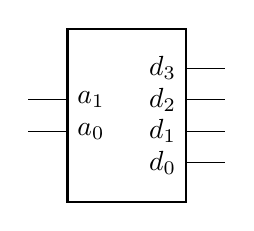
\begin{tikzpicture}
\pgfmathsetmacro{\kpin}{0.5}
\pgfmathsetmacro{\kpsep}{0.40}
\pgfmathsetmacro{\kul}{0.50}
\pgfmathsetmacro{\kxdim}{1.5}
\pgfmathsetmacro{\kydim}{2*\kul+3*\kpsep}
\draw[thick](0,0) rectangle ++(\kxdim,\kydim);
\foreach \y/\a in {1/{a_0},2/{a_1}}{\draw(0,\kul+\y*\kpsep)node[right]{$\a$}--++(-\kpin,0);}
\foreach \y/\d in {0/{d_0},1/{d_1},2/{d_2},3/{d_3}}{\draw(\kxdim,\kul+\y*\kpsep)node[left]{$\d$}--++(\kpin,0);}
\end{tikzpicture}
\end{subfigure}\hfill
\begin{subfigure}{0.6\textwidth}
\centering
\begin{otherlanguage}{english}
\begin{tabular}{CC|CCCC}
\toprule
\multicolumn{2}{c|}{\text{\RL{داخلی بِٹ}}}&\multicolumn{4}{c}{\text{\RL{خارجی بِٹ}}}\\
a_0&a_0&d_3&d_2&d_1&d_0\\
\midrule
0&0&0&0&0&1\\
0&1&0&0&1&0\\
1&0&0&1&0&0\\
1&1&1&0&0&0\\
\bottomrule
\end{tabular}
\end{otherlanguage}
\end{subfigure}
\caption{دو سے چار شناخت کار}
\label{شکل_ترکیبی_دو_چار_شناخت_کار}
\end{figure}
شکل \حوالہ{شکل_ترکیبی_دو_چار_شناخت_کار} میں دو سے چار شناخت کار کی علامت اور کارکردگی کا جدول پیش ہیں۔داخلی بِٹوں کی ہر منفرد ترتیب، خارجی بِٹوں میں سے ایک منفرد بِٹ منتخب کرتی ہے۔یہاں چنی گئی بِٹ بلند کی گئی ہے، شناخت کار یوں بھی تشکیل دی جا سکتی ہے کہ منتخب بِٹ پست ہو۔

 مداخل \عددی{00} (جدول کی پہلی صف) کرنے سے چار مخارج میں سے ایک، یعنی \عددی{d_0} کی شناخت ہوتی ہے۔اسی طرح \عددی{01} مخارج \عددی{d_1} کی، \عددی{10} مخارج \عددی{d_2} کی ، اور \عددی{11}مخارج \عددی{d_3} کی شناخت کرتے ہیں۔
 
 اگر \عددی{d} چار مختلف جگہیں، مثلاً، چار گلیاں، یا چار مکان، تصور کی جائیں، تب \عددی{a} ان کا پتہ ہو گا، جس کے ذریعہ ان تک پہنچنا ممکن ہو گا۔ اسی مشابہت سے \عددی{a} کو \اصطلاح{پتہ کے بِٹ} یا \اصطلاح{پتہ بِٹ}\فرہنگ{پتہ بِٹ}\حاشیہب{address bits}\فرہنگ{address bits} یا صرف \اصطلاح{پتہ}\فرہنگ{پتہ}\حاشیہب{address}\فرہنگ{address} کہتے ہیں۔عددی برقیات میں اس طرح جگہ تعین کرنے والے \قول{پتہ کے بِٹوں} کا استعمال عام ہے اور انہیں، عموماً، \عددی{a}سے ظاہر کیا جاتا ہے۔

کسی بھی پتہ کو اعشاری روپ میں لکھیں؛ یہی مقام منتخب ہو گا۔ یوں \عددی{101_2} پتہ مقام \عددی{5_{10}} یعنی \عددی{d_5} منتخب کرے گا۔



شکل \حوالہ{شکل_ترکیبی_دو_چار_شناخت_کار} میں دیے جدول کو مخارج کے لئے حل کر کے درج ذیل حاصل ہوں گے۔
\begin{align*}
d_0&=\overline{a}_1\overline{a}_0\\
d_1&=\overline{a}_1a_0\\
d_2&=a_1\overline{a}_0\\
d_3&=a_1a_0
\end{align*}

شکل \حوالہ{شکل_ترکیبی_دو_با_چار_شناخت_کار} میں ان مساوات سے حاصل دو با چار \عددی{(2\times 4)} \اصطلاح{ شناخت کار پیش}\فرہنگ{شناخت کار}\حاشیہب{decoder}\فرہنگ{decoder} ہے، جس کے داخلی بِٹ کی تعداد دو \عددی{(2)}، جبکہ خارجی بِٹ کی تعداد چار \عددی{(4)} ہے۔ 
\begin{figure}
\centering
\begin{tikzpicture}
\pgfmathsetmacro{\kpin}{0.5}
\pgfmathsetmacro{\kxsep}{4}
\pgfmathsetmacro{\kysep}{1.25}
\pgfmathsetmacro{\kysepa}{1.5}
\pgfmathsetmacro{\kxa}{0.5}
\pgfmathsetmacro{\kxb}{0.75}
\pgfmathsetmacro{\kxc}{1}
\pgfmathsetmacro{\kxd}{1.25}
\draw(0,\kysepa) node[not port,scale=1](u1){};
\draw(0,0)node[not port, scale=1](u2){};
\draw(\kxsep,-\kysep)node[and port, scale=1,number inputs=2](u3){};
\draw(\kxsep,-2*\kysep)node[and port, scale=1,number inputs=2](u4){};
\draw(\kxsep,-3*\kysep)node[and port, scale=1,number inputs=2](u5){};
\draw(\kxsep,-4*\kysep)node[and port, scale=1,number inputs=2](u6){};
\draw(u6.in 1)--++(-\kxa,0)coordinate(aa) |-coordinate(bb)(u1.out)node[above]{$\overline{a}_1$};
\draw($(aa)!(u5.in 1)!(bb)$)--(u5.in 1);
\draw(u1.in)--++(0,-\kysepa/2)coordinate(cc) (u1.in)--++(-\kpin,0)node[left]{$a_1$}; 
\draw(u4.in 1)--++(-\kxb,0) |-(cc);
\draw(u3.in 1)--++(-\kxb,0);
\draw(u6.in 2)--++(-\kxc,0) |-(u2.out)node[above]{$\overline{a}_0$} (u4.in 2)--++(-\kxc,0);
\draw(u3.in 2)-|coordinate(ff)(u2.in)--++(-\kpin,0)node[left]{$a_0$};
\draw(u5.in 2)--++(-\kxd,0)coordinate(gg)--($(u3.in 2)!(gg)!(ff)$);
\draw(u6.out)node[right]{$d_0$};
\draw(u5.out)node[right]{$d_1$};
\draw(u4.out)node[right]{$d_2$};
\draw(u3.out)node[right]{$d_3$};
\end{tikzpicture}
\caption{دو با چار شناخت کار}
\label{شکل_ترکیبی_دو_با_چار_شناخت_کار}
\end{figure}

شکل \حوالہ{شکل_ترکیبی_دو_با_چار_شناخت_کار} میں پیش شناخت کار کے تمام ضرب گیٹوں کے ساتھ اضافی قابو مداخل جوڑ کر مجاز و معذور صلاحیت کا \عددی{(2\times 4)} شناخت کار حاصل ہو گا، جو شکل \حوالہ{شکل_ترکیبی_مجازومعذور_شناخت_کار} میں پیش ہے۔ شناخت کار، بلند قابو اشارہ \عددی{(e)} کی صورت میں، شناخت کرنے کا مجاذ ہو گا، پست اشارے کی صورت میں شناخت کار معذور ہو گا اور اس کے تمام مخارج پست ہوں گے۔ شکل-ب میں اس کی علامت پیش کی گئی ہے، جہاں قابو اشارہ کو مختصراً \قول{مجاز} کہا گیا ہے۔

\begin{figure}
\centering
\begin{subfigure}{0.6\textwidth}
\centering
\begin{tikzpicture}
\pgfmathsetmacro{\kpin}{0.5}
\pgfmathsetmacro{\kxsep}{4}
\pgfmathsetmacro{\kysep}{1.25}
\pgfmathsetmacro{\kysepa}{1.5}
\pgfmathsetmacro{\kxa}{0.5}
\pgfmathsetmacro{\kxb}{0.75}
\pgfmathsetmacro{\kxc}{1}
\pgfmathsetmacro{\kxd}{1.25}
\draw(0,\kysepa) node[not port,scale=1](u1){};
\draw(0,0)node[not port, scale=1](u2){};
\draw(\kxsep,-\kysep)node[and port, scale=1,number inputs=3](u3){};
\draw(\kxsep,-2*\kysep)node[and port, scale=1,number inputs=3](u4){};
\draw(\kxsep,-3*\kysep)node[and port, scale=1,number inputs=3](u5){};
\draw(\kxsep,-4*\kysep)node[and port, scale=1,number inputs=3](u6){};
\draw(u6.in 1)--++(-\kxa,0)coordinate(aa) |-coordinate(bb)(u1.out)node[above]{$\overline{a}_1$};
\draw($(aa)!(u5.in 1)!(bb)$)--(u5.in 1);
\draw(u1.in)--++(0,-\kysepa/2)coordinate(cc) (u1.in)--++(-\kpin,0)node[left]{$a_1$}; 
\draw(u4.in 1)--++(-\kxb,0) |-(cc);
\draw(u3.in 1)--++(-\kxb,0);
\draw(u6.in 2)--++(-\kxc,0) |-(u2.out)node[above]{$\overline{a}_0$} (u4.in 2)--++(-\kxc,0);
\draw(u3.in 2)-|coordinate(ff)(u2.in)--++(-\kpin,0)node[left]{$a_0$};
\draw(u5.in 2)--++(-\kxd,0)coordinate(gg)--($(u3.in 2)!(gg)!(ff)$);
\draw(u6.out)node[right]{$d_0$};
\draw(u5.out)node[right]{$d_1$};
\draw(u4.out)node[right]{$d_2$};
\draw(u3.out)node[right]{$d_3$};
\draw(u3.in 3)--(u6.in 3)--++(-\kxsep+\kpin,0)node[below]{$e$}node[above]{$\text{مجاز}/\overline{\text{معذور}}$};
\end{tikzpicture}
\caption{}
\end{subfigure}\hfill
\begin{subfigure}{0.40\textwidth}
\centering
\begin{tikzpicture}
\pgfmathsetmacro{\kpin}{0.5}
\pgfmathsetmacro{\kpsep}{0.40}
\pgfmathsetmacro{\kul}{0.50}
\pgfmathsetmacro{\kxdim}{1.5}
\pgfmathsetmacro{\kydim}{2*\kul+3*\kpsep}
\draw[thick](0,0) rectangle ++(\kxdim,\kydim);
\foreach \y/\a in {0/e,2/{a_0},3/{a_1}}{\draw(0,\kul+\y*\kpsep)node[right]{$\a$}--++(-\kpin,0);}
\foreach \y/\d in {0/{d_0},1/{d_1},2/{d_2},3/{d_3}}{\draw(\kxdim,\kul+\y*\kpsep)node[left]{$\d$}--++(\kpin,0);}
\draw(0,\kul)node[above left]{مجاز};
\end{tikzpicture}
\caption{}
\end{subfigure}
\caption{مجاز و معذور صلاحیت کا دو با چار شناخت کار}
\label{شکل_ترکیبی_مجازومعذور_شناخت_کار}
\end{figure}


\begin{table}
\caption{مجاز و معذور صلاحیت کا شناخت کار}
\label{جدول_ترکیبی_مجازومعذار_شناخت_کار}
\centering
\begin{subtable}{0.45\textwidth}
\caption{}
\centering
\begin{otherlanguage}{english}
\begin{tabular}{CCC|CCCC}
\toprule
e&a_1&a_0&d_3&d_2&d_1&d_0\\
\midrule
0&0&0&0&0&0&0\\
0&0&1&0&0&0&0\\
0&1&0&0&0&0&0\\
0&1&1&0&0&0&0\\
1&0&0&0&0&0&1\\
1&0&1&0&0&1&0\\
1&1&0&0&1&0&0\\
1&1&1&1&0&0&0\\
\bottomrule
\end{tabular}
\end{otherlanguage}
\end{subtable}\hfill
\begin{subtable}{0.45\textwidth}
\caption{}
\centering
\begin{otherlanguage}{english}
\begin{tabular}{CCC|CCCC}
\toprule
e&a_1&a_0&d_3&d_2&d_1&d_0\\
\midrule
0&x&x&0&0&0&0\\
1&0&0&0&0&0&1\\
1&0&1&0&0&1&0\\
1&1&0&0&1&0&0\\
1&1&1&1&0&0&0\\
\bottomrule
\end{tabular}
\end{otherlanguage}
\end{subtable}
\end{table}

 جدول \حوالہ{جدول_ترکیبی_مجازومعذار_شناخت_کار}-الف میں مجاز و معذور صلاحیت کے شناخت کار کی کارکردگی پیش کی گئی ہے۔اس جدول کو مختصراً جدول-ب کی صورت میں پیش کیا جاتا ہے، جہاں پہلی صف میں قابو اشارہ پست \عددی{(e=0)} ہے لہٰذا \عددی{a_0} اور \عددی{a_1} کی قیمتیں اہمیت نہیں رکھتی؛ یوں پہلی صف میں \عددی{a_0} اور \عددی{a_1} کی قیمت \عددی{x} لکھی جاتی ہے۔ 


\begin{table}
\caption{بلند عمل پیرا، تین با آٹھ شناخت کار}
\label{جدول_ترکیبی_تین_با_آٹھ_شناخت_کار}
\centering
\begin{otherlanguage}{english}
\begin{tabular}{CCC|CCCCCCCC}
\toprule
a_2&a_1&a_0&d_7&d_6&d_5&d_4&d_3&d_2&d_1&d_0\\
\midrule
0&0&0&0&0&0&0&0&0&0&1\\
0&0&1&0&0&0&0&0&0&1&0\\
0&1&0&0&0&0&0&0&1&0&0\\
0&1&1&0&0&0&0&1&0&0&0\\
1&0&0&0&0&0&1&0&0&0&0\\
1&0&1&0&0&1&0&0&0&0&0\\
1&1&0&0&1&0&0&0&0&0&0\\
1&1&1&1&0&0&0&0&0&0&0\\
\bottomrule
\end{tabular}
\end{otherlanguage}
\end{table}

تین با آٹھ \عددی{(3\times 8)} شناخت کار کا دور حاصل کرنے کی خاطر، تین مداخل کا ایسا جدول لکھتے ہیں جس میں مداخل کی ہر ترتیب ایک منفرد مخارج
 منتخب کرے ( جدول \حوالہ{جدول_ترکیبی_تین_با_آٹھ_شناخت_کار} دیکھیں)۔چونکہ چنُا گیا مخارج بلند ہو گا، لہٰذا ایسا شناخت کار، \اصطلاح{ بلند عمل پیرا}\فرہنگ{عمل پیرا!بلند}\حاشیہب{active high}\فرہنگ{active!high} کہلاتا ہے۔مخارج تفاعلات کی مساوات، مجموعہ ارکان ضرب کی صورت میں حاصل کرتے ہیں۔
\begin{align*}
d_0&=\overline{a}_2 \overline{a}_1 \overline{a}_0\\
d_1&=\overline{a}_2 \overline{a}_1 a_0\\
d_2&=\overline{a}_2 a_1 \overline{a}_0\\
d_3&=\overline{a}_2 a_1 a_0\\
d_4&=a_2\, \overline{a}_1 \overline{a}_0\\
d_5&=a_2\, \overline{a}_1 a_0\\
d_6&=a_2\, a_1\, \overline{a}_0\\
d_7&=a_2\, a_1\, a_0
\end{align*}
ان تفاعلات سے حاصل، بلند عمل پیرا، تین با آٹھ \عددی{(3\times 8)} شناخت کار شکل \حوالہ{شکل_ترکیبی_تین_با_آٹھ_شناخت_کار} میں پیش ہے۔
\begin{figure}
\centering
\begin{tikzpicture}
\pgfmathsetmacro{\kxs}{1.25}
\pgfmathsetmacro{\kxsa}{1.5}
\pgfmathsetmacro{\kstep}{0.25}
\pgfmathsetmacro{\kbase}{0.5}
\pgfmathsetmacro{\kys}{\kbase+5*\kstep}
\pgfmathsetmacro{\kpin}{0.5}
\pgfmathsetmacro{\kpina}{\kxsa/2}
\draw(0*\kxs,0)node[and port,scale=1,number inputs=3,rotate=-90,anchor=in 1](u7){};
\draw(1*\kxs,0)node[and port,scale=1,number inputs=3,rotate=-90,anchor=in 1](u6){};
\draw(2*\kxs,0)node[and port,scale=1,number inputs=3,rotate=-90,anchor=in 1](u5){};
\draw(3*\kxs,0)node[and port,scale=1,number inputs=3,rotate=-90,anchor=in 1](u4){};
\draw(4*\kxs,0)node[and port,scale=1,number inputs=3,rotate=-90,anchor=in 1](u3){};
\draw(5*\kxs,0)node[and port,scale=1,number inputs=3,rotate=-90,anchor=in 1](u2){};
\draw(6*\kxs,0)node[and port,scale=1,number inputs=3,rotate=-90,anchor=in 1](u1){};
\draw(7*\kxs,0)node[and port,scale=1,number inputs=3,rotate=-90,anchor=in 1](u0){};
\draw(0.5,\kys)node[not port,scale=0.9,rotate=-90,anchor=out](u8){};
\draw(0.5-\kxsa,\kys)node[not port,scale=0.9,rotate=-90,anchor=out](u9){};
\draw(0.5-2*\kxsa,\kys)node[not port,scale=0.9,rotate=-90,anchor=out](u10){};
\draw(u8.in)--++(0,\kpin)node[above]{$a_0$};
\draw(u9.in)--++(0,\kpin)node[above]{$a_1$};
\draw(u10.in)--++(0,\kpin)node[above]{$a_2$};
\draw(u0.out)node[below]{$d_0$} (u1.out)node[below]{$d_1$} (u2.out)node[below]{$d_2$} 
(u3.out)node[below]{$d_3$} (u4.out)node[below]{$d_4$} (u5.out)node[below]{$d_5$}
(u6.out)node[below]{$d_6$} (u7.out)node[below]{$d_7$};
\draw(u8.in)--++(-\kpina,0)coordinate(kin8);
\draw(u9.in)--++(-\kpina,0)coordinate(kin9);
\draw(u10.in)--++(-\kpina,0)coordinate(kin10);
\draw(u0.in 1)++(\kpin/2,\kbase+0*\kstep)-|(kin10);
\draw(u0.in 1)++(\kpin/2,\kbase+1*\kstep)-|(u10.out);
\draw(u0.in 1)++(\kpin/2,\kbase+2*\kstep)-|(kin9);
\draw(u0.in 1)++(\kpin/2,\kbase+3*\kstep)-|(u9.out);
\draw(u0.in 1)++(\kpin/2,\kbase+4*\kstep)-|(kin8);
\draw(u0.in 1)++(\kpin/2,\kbase+5*\kstep)-|(u8.out);
\draw(u0.in 1)--++(0,\kbase+5*\kstep) (u0.in 2)--++(0,\kbase+3*\kstep) (u0.in 3)--++(0,\kbase+1*\kstep);
\draw(u1.in 1)--++(0,\kbase+4*\kstep) (u1.in 2)--++(0,\kbase+3*\kstep) (u1.in 3)--++(0,\kbase+1*\kstep);
\draw(u2.in 1)--++(0,\kbase+5*\kstep) (u2.in 2)--++(0,\kbase+2*\kstep) (u2.in 3)--++(0,\kbase+1*\kstep);
\draw(u3.in 1)--++(0,\kbase+4*\kstep) (u3.in 2)--++(0,\kbase+2*\kstep) (u3.in 3)--++(0,\kbase+1*\kstep);
\draw(u4.in 1)--++(0,\kbase+5*\kstep) (u4.in 2)--++(0,\kbase+3*\kstep) (u4.in 3)--++(0,\kbase+0*\kstep);
\draw(u5.in 1)--++(0,\kbase+4*\kstep) (u5.in 2)--++(0,\kbase+3*\kstep) (u5.in 3)--++(0,\kbase+0*\kstep);
\draw(u6.in 1)--++(0,\kbase+5*\kstep) (u6.in 2)--++(0,\kbase+2*\kstep) (u6.in 3)--++(0,\kbase+0*\kstep);
\draw(u7.in 1)--++(0,\kbase+4*\kstep) (u7.in 2)--++(0,\kbase+2*\kstep) (u7.in 3)--++(0,\kbase+0*\kstep);
\end{tikzpicture}
\caption{بلند عمل پیرا، تین با آٹھ \عددی{(3\times 8)} شناخت کار}
\label{شکل_ترکیبی_تین_با_آٹھ_شناخت_کار}
\end{figure}


اس میں مجاز مداخل کا اضافہ کرنے سے مجاز و معذور صلاحیت، بلند عمل پیرا، تین با آٹھ شناخت کار حاصل ہو گا جو شکل \حوالہ{شکل_ترکیبی_تین_با_آٹھ_مجاز_شناخت_کار} میں پیش ہے۔ مجاز بلند ہونے کی صورت میں شناخت کار کام کرے گا، جبکہ پست مجاز کی صورت میں تمام مخارج پست رہیں گے؛ ہم کہتے ہیں یہ \اصطلاح{بلند مجاز}\فرہنگ{مجاز!بلند}\حاشیہب{active high}\فرہنگ{active!high} شناخت کار ہے۔ جدول \حوالہ{جدول_ترکیبی_مجاز_تین_با_آٹھ_شناخت_کار} میں اس کی کارکردگی پیش کی گئی ہے۔ پہلی صف میں \عددی{e} پست ہے، لہٰذا، شناخت کار معذور ہو گا، اور اس کے تین مداخل \عددی{a_0}، \عددی{a_1}، اور \عددی{a_2} کی قیمتیں اہمیت نہیں رکھتی؛ اسی لئے انہیں \عددی{x} لکھا گیا ہے جو \عددی{0} یا \عددی{1} ہو سکتا ہے۔ یہ (پہلی) صف درحقیقت، \عددی{a_2a_1a_0} کی آٹھ \عددی{(8)} قیمتوں، \عددی{000_2} تا \عددی{111_2}، لہٰذا، آٹھ صفوں کو ظاہر کرتی ہے۔
\begin{figure}
\centering
\begin{tikzpicture}
\pgfmathsetmacro{\kxs}{1.25}
\pgfmathsetmacro{\kxsa}{1.5}
\pgfmathsetmacro{\kstep}{0.25}
\pgfmathsetmacro{\kbase}{1}
\pgfmathsetmacro{\kys}{\kbase+5*\kstep}
\pgfmathsetmacro{\kpin}{0.5}
\pgfmathsetmacro{\kpina}{\kxsa/2}
\draw(0*\kxs,0)node[and port,scale=1,number inputs=4,rotate=-90,anchor=in 1](u7){};
\draw(1*\kxs,0)node[and port,scale=1,number inputs=4,rotate=-90,anchor=in 1](u6){};
\draw(2*\kxs,0)node[and port,scale=1,number inputs=4,rotate=-90,anchor=in 1](u5){};
\draw(3*\kxs,0)node[and port,scale=1,number inputs=4,rotate=-90,anchor=in 1](u4){};
\draw(4*\kxs,0)node[and port,scale=1,number inputs=4,rotate=-90,anchor=in 1](u3){};
\draw(5*\kxs,0)node[and port,scale=1,number inputs=4,rotate=-90,anchor=in 1](u2){};
\draw(6*\kxs,0)node[and port,scale=1,number inputs=4,rotate=-90,anchor=in 1](u1){};
\draw(7*\kxs,0)node[and port,scale=1,number inputs=4,rotate=-90,anchor=in 1](u0){};
\draw(0.5,\kys)node[not port,scale=1,rotate=-90,anchor=out](u8){};
\draw(0.5-\kxsa,\kys)node[not port,scale=1,rotate=-90,anchor=out](u9){};
\draw(0.5-2*\kxsa,\kys)node[not port,scale=1,rotate=-90,anchor=out](u10){};
\draw(u8.in)--++(0,\kpin)node[above]{$a_0$};
\draw(u9.in)--++(0,\kpin)node[above]{$a_1$};
\draw(u10.in)--++(0,\kpin)node[above]{$a_2$};
\draw(u0.out)node[below]{$d_0$} (u1.out)node[below]{$d_1$} (u2.out)node[below]{$d_2$} 
(u3.out)node[below]{$d_3$} (u4.out)node[below]{$d_4$} (u5.out)node[below]{$d_5$}
(u6.out)node[below]{$d_6$} (u7.out)node[below]{$d_7$};
\draw(u8.in)--++(-\kpina,0)coordinate(kin8);
\draw(u9.in)--++(-\kpina,0)coordinate(kin9);
\draw(u10.in)--++(-\kpina,0)coordinate(kin10);
\draw(u0.in 1)++(\kpin/2,\kbase+0*\kstep)-|(kin10);
\draw(u0.in 1)++(\kpin/2,\kbase-2*\kstep)-|coordinate(ken)(u7.in 4) (ken)--++(-4*\kpin,0)node[left]{$e$}node[below,xshift=0.5em,yshift=-0.25em]{مجاز};
\draw(u0.in 1)++(\kpin/2,\kbase+1*\kstep)-|(u10.out);
\draw(u0.in 1)++(\kpin/2,\kbase+2*\kstep)-|(kin9);
\draw(u0.in 1)++(\kpin/2,\kbase+3*\kstep)-|(u9.out);
\draw(u0.in 1)++(\kpin/2,\kbase+4*\kstep)-|(kin8);
\draw(u0.in 1)++(\kpin/2,\kbase+5*\kstep)-|(u8.out);
\draw(u0.in 1)--++(0,\kbase+5*\kstep) (u0.in 2)--++(0,\kbase+3*\kstep) (u0.in 3)--++(0,\kbase+1*\kstep);
\draw(u1.in 1)--++(0,\kbase+4*\kstep) (u1.in 2)--++(0,\kbase+3*\kstep) (u1.in 3)--++(0,\kbase+1*\kstep);
\draw(u2.in 1)--++(0,\kbase+5*\kstep) (u2.in 2)--++(0,\kbase+2*\kstep) (u2.in 3)--++(0,\kbase+1*\kstep);
\draw(u3.in 1)--++(0,\kbase+4*\kstep) (u3.in 2)--++(0,\kbase+2*\kstep) (u3.in 3)--++(0,\kbase+1*\kstep);
\draw(u4.in 1)--++(0,\kbase+5*\kstep) (u4.in 2)--++(0,\kbase+3*\kstep) (u4.in 3)--++(0,\kbase+0*\kstep);
\draw(u5.in 1)--++(0,\kbase+4*\kstep) (u5.in 2)--++(0,\kbase+3*\kstep) (u5.in 3)--++(0,\kbase+0*\kstep);
\draw(u6.in 1)--++(0,\kbase+5*\kstep) (u6.in 2)--++(0,\kbase+2*\kstep) (u6.in 3)--++(0,\kbase+0*\kstep);
\draw(u7.in 1)--++(0,\kbase+4*\kstep) (u7.in 2)--++(0,\kbase+2*\kstep) (u7.in 3)--++(0,\kbase+0*\kstep);
\draw(u0.in 4)--++(0,\kbase-2*\kstep) (u1.in 4)--++(0,\kbase-2*\kstep) (u2.in 4)--++(0,\kbase-2*\kstep)
(u3.in 4)--++(0,\kbase-2*\kstep) (u4.in 4)--++(0,\kbase-2*\kstep) 
(u5.in 4)--++(0,\kbase-2*\kstep) (u6.in 4)--++(0,\kbase-2*\kstep);
\end{tikzpicture}
\caption{بلند مجاز، بلند عمل پیرا، تین با آٹھ شناخت کار}
\label{شکل_ترکیبی_تین_با_آٹھ_مجاز_شناخت_کار}
\end{figure}
%
\begin{table}
\caption{بلند مجاز، بلند عمل پیرا، تین با آٹھ شناخت کار}
\label{جدول_ترکیبی_مجاز_تین_با_آٹھ_شناخت_کار}
\centering
\begin{otherlanguage}{english}
\begin{tabular}{CCCC|CCCCCCCC}
\toprule
e&a_2&a_1&a_0&d_7&d_6&d_5&d_4&d_3&d_2&d_1&d_0\\
\midrule
0&x&x&x&0&0&0&0&0&0&0&0\\
1&0&0&0&0&0&0&0&0&0&0&1\\
1&0&0&1&0&0&0&0&0&0&1&0\\
1&0&1&0&0&0&0&0&0&1&0&0\\
1&0&1&1&0&0&0&0&1&0&0&0\\
1&1&0&0&0&0&0&1&0&0&0&0\\
1&1&0&1&0&0&1&0&0&0&0&0\\
1&1&1&0&0&1&0&0&0&0&0&0\\
1&1&1&1&1&0&0&0&0&0&0&0\\
\bottomrule
\end{tabular}
\end{otherlanguage}
\end{table}
\ابتدا{مشق}
شکل \حوالہ{شکل_ترکیبی_تین_با_آٹھ_مجاز_شناخت_کار} میں دایاں جمع گیٹ کا مخارج کیا ہے؟ باقی مخارج بھی شکل سے حاصل کریں۔ کیا یہ جدول \حوالہ{جدول_ترکیبی_تین_با_آٹھ_شناخت_کار} پر پورا اترتے ہیں؟
\انتہا{مشق}

بعض اوقات، ایسے شناخت کار کی ضرورت پیش آتی ہے جس کا چنا گیا مخارج پست ہو۔ایسا شناخت کار،\اصطلاح{پست عمل پیرا}\فرہنگ{عمل پیرا!پست}\حاشیہب{active low}\فرہنگ{active!low} کہلاتا ہے۔ جدول \حوالہ{جدول_ترکیبی_مجاز__پست_عمل_پیرا_تین_با_آٹھ_شناخت_کار} میں ایسا پست عمل پیرا، تین با آٹھ شناخت کار پیش ہے، جو قابو اشارہ \عددی{\overline{\text{مجاز}}} پست ہونے کی صورت میں کام کرتا ہے؛ ہم کہتے ہیں یہ \اصطلاح{پست مجاز}\فرہنگ{مجاز!پست}\حاشیہب{active low}\فرہنگ{active!low} ہے۔ روایتاً، پست عمل پیرا مخارج کو \عددی{\overline{y}} سے ظاہر کیا جاتا ہے، جہاں بِٹ پر \قول{لکیر} اس بات کی یاد دہانی کراتی ہے کہ چنا گیا مخارج پست ہو گا۔ قابو اشارہ پر بھی \قول{لکیر} کھینچی گئی ہے \عددی{(\overline{e})} جو اس حقیقت کو ظاہر کرتی ہے کہ شناخت کار اس صورت کام کرے گا جب قابو اشارہ پست کیا جائے۔ شکل \حوالہ{شکل_ترکیبی_تین_با_آٹھ_پست_عمل_پیرا_شناخت_کار} میں اس کا دور پیش ہے، جو 
شکل \حوالہ{شکل_ترکیبی_تین_با_آٹھ_مجاز_شناخت_کار} میں ضرب گیٹ کی جگہ متمم ضرب گیٹ ڈالنے سے، اور قابو اشارہ کے ساتھ نفی گیٹ منسلک کرنے سے حاصل ہو گا۔
 
\begin{table}
\caption{پست مجاز، پست عمل پیرا، تین با آٹھ شناخت کار}
\label{جدول_ترکیبی_مجاز__پست_عمل_پیرا_تین_با_آٹھ_شناخت_کار}
\centering
\begin{otherlanguage}{english}
\begin{tabular}{CCCC|CCCCCCCC}
\toprule
\overline{e}&a_2&a_1&a_0&\overline{y}_7&\overline{y}_6&\overline{y}_5&\overline{y}_4&\overline{y}_3&
\overline{y}_2&\overline{y}_1&\overline{y}_0\\
\midrule
1&x&x&x&1&1&1&1&1&1&1&1\\
0&0&0&0&1&1&1&1&1&1&1&0\\
0&0&0&1&1&1&1&1&1&1&0&1\\
0&0&1&0&1&1&1&1&1&0&1&1\\
0&0&1&1&1&1&1&1&0&1&1&1\\
0&1&0&0&1&1&1&0&1&1&1&1\\
0&1&0&1&1&1&0&1&1&1&1&1\\
0&1&1&0&1&0&1&1&1&1&1&1\\
0&1&1&1&0&1&1&1&1&1&1&1\\
\bottomrule
\end{tabular}
\end{otherlanguage}
\end{table}
%
\begin{figure}
\centering
\begin{tikzpicture}
\pgfmathsetmacro{\kxs}{1.25}
\pgfmathsetmacro{\kxsa}{1.5}
\pgfmathsetmacro{\kstep}{0.25}
\pgfmathsetmacro{\kbase}{1}
\pgfmathsetmacro{\kys}{\kbase+5*\kstep}
\pgfmathsetmacro{\kpin}{0.5}
\pgfmathsetmacro{\kpina}{\kxsa/2}
\pgfmathsetmacro{\ke}{\kbase-2.5*\kstep}
\draw(0*\kxs,0)node[nand port,scale=1,number inputs=4,rotate=-90,anchor=in 1](u7){};
\draw(1*\kxs,0)node[nand port,scale=1,number inputs=4,rotate=-90,anchor=in 1](u6){};
\draw(2*\kxs,0)node[nand port,scale=1,number inputs=4,rotate=-90,anchor=in 1](u5){};
\draw(3*\kxs,0)node[nand port,scale=1,number inputs=4,rotate=-90,anchor=in 1](u4){};
\draw(4*\kxs,0)node[nand port,scale=1,number inputs=4,rotate=-90,anchor=in 1](u3){};
\draw(5*\kxs,0)node[nand port,scale=1,number inputs=4,rotate=-90,anchor=in 1](u2){};
\draw(6*\kxs,0)node[nand port,scale=1,number inputs=4,rotate=-90,anchor=in 1](u1){};
\draw(7*\kxs,0)node[nand port,scale=1,number inputs=4,rotate=-90,anchor=in 1](u0){};
\draw(0.5,\kys)node[not port,scale=1,rotate=-90,anchor=out](u8){};
\draw(0.5-\kxsa,\kys)node[not port,scale=1,rotate=-90,anchor=out](u9){};
\draw(0.5-2*\kxsa,\kys)node[not port,scale=1,rotate=-90,anchor=out](u10){};
\draw(u8.in)--++(0,\kpin)node[above]{$a_0$};
\draw(u9.in)--++(0,\kpin)node[above]{$a_1$};
\draw(u10.in)--++(0,\kpin)node[above]{$a_2$};
\draw(u0.out)node[below]{$d_0$} (u1.out)node[below]{$d_1$} (u2.out)node[below]{$d_2$} 
(u3.out)node[below]{$d_3$} (u4.out)node[below]{$d_4$} (u5.out)node[below]{$d_5$}
(u6.out)node[below]{$d_6$} (u7.out)node[below]{$d_7$};
\draw(u8.in)--++(-\kpina,0)coordinate(kin8);
\draw(u9.in)--++(-\kpina,0)coordinate(kin9);
\draw(u10.in)--++(-\kpina,0)coordinate(kin10);
\draw(u0.in 1)++(\kpin/2,\kbase+0*\kstep)-|(kin10);
\draw(u0.in 1)++(\kpin/2,\ke)-|coordinate(ken)(u7.in 4) (ken)--++(-0.25*\kpin,0)
node[not port,scale=1,anchor=out](u11){} (u11.in)node[left]{$\overline{e}$}node[below,xshift=-0.5em,yshift=-0.5em]{$\overline{\text{مجاز}}$};
\draw(u0.in 1)++(\kpin/2,\kbase+1*\kstep)-|(u10.out);
\draw(u0.in 1)++(\kpin/2,\kbase+2*\kstep)-|(kin9);
\draw(u0.in 1)++(\kpin/2,\kbase+3*\kstep)-|(u9.out);
\draw(u0.in 1)++(\kpin/2,\kbase+4*\kstep)-|(kin8);
\draw(u0.in 1)++(\kpin/2,\kbase+5*\kstep)-|(u8.out);
\draw(u0.in 1)--++(0,\kbase+5*\kstep) (u0.in 2)--++(0,\kbase+3*\kstep) (u0.in 3)--++(0,\kbase+1*\kstep);
\draw(u1.in 1)--++(0,\kbase+4*\kstep) (u1.in 2)--++(0,\kbase+3*\kstep) (u1.in 3)--++(0,\kbase+1*\kstep);
\draw(u2.in 1)--++(0,\kbase+5*\kstep) (u2.in 2)--++(0,\kbase+2*\kstep) (u2.in 3)--++(0,\kbase+1*\kstep);
\draw(u3.in 1)--++(0,\kbase+4*\kstep) (u3.in 2)--++(0,\kbase+2*\kstep) (u3.in 3)--++(0,\kbase+1*\kstep);
\draw(u4.in 1)--++(0,\kbase+5*\kstep) (u4.in 2)--++(0,\kbase+3*\kstep) (u4.in 3)--++(0,\kbase+0*\kstep);
\draw(u5.in 1)--++(0,\kbase+4*\kstep) (u5.in 2)--++(0,\kbase+3*\kstep) (u5.in 3)--++(0,\kbase+0*\kstep);
\draw(u6.in 1)--++(0,\kbase+5*\kstep) (u6.in 2)--++(0,\kbase+2*\kstep) (u6.in 3)--++(0,\kbase+0*\kstep);
\draw(u7.in 1)--++(0,\kbase+4*\kstep) (u7.in 2)--++(0,\kbase+2*\kstep) (u7.in 3)--++(0,\kbase+0*\kstep);
%
\draw(u0.in 4)--++(0,\ke) (u1.in 4)--++(0,\ke) (u2.in 4)--++(0,\ke) (u3.in 4)--++(0,\ke) (u4.in 4)--++(0,\ke) 
(u5.in 4)--++(0,\ke) (u6.in 4)--++(0,\ke);
\end{tikzpicture}
\caption{پست مجاز، پست عمل پیرا، تین با آٹھ شناخت کار}
\label{شکل_ترکیبی_تین_با_آٹھ_پست_عمل_پیرا_شناخت_کار}
\end{figure}

شکل \حوالہ{شکل_ترکیبی_بلند_پست_علامت_شناخت_کار} میں تین با آٹھ شناخت کار کی علامتیں پیش ہیں۔شکل -الف میں بلند مجاز، بلند عمل پیرا، شکل-ب میں پست مجاز، بلند عمل پیرا اور شکل-ج میں پست مجاز، پست عمل پیرا روپ دکھائے گئے ہیں۔ ان علامتوں میں خارجی پنیوں پر گول دائرہ اس بات کی یقین دہانی کراتا ہے کہ منتخب ہونے کی صورت میں یہ بِٹ پست ہو گی۔ اسی طرح قابو بِٹ پر گول دائرہ یاد دہانی کراتا ہے کہ شناخت کار صرف اس صورت مجاز ہو گا جب یہ اشارہ پست ہو۔
\begin{figure}
\centering
\begin{subfigure}{0.30\textwidth}
\centering
\begin{tikzpicture}
\pgfmathsetmacro{\kpin}{0.5}
\pgfmathsetmacro{\kpsep}{0.40}
\pgfmathsetmacro{\kul}{0.50}
\pgfmathsetmacro{\kxdim}{1.5}
\pgfmathsetmacro{\kydim}{2*\kul+7*\kpsep}
\draw[thick](0,0) rectangle ++(\kxdim,\kydim);
\foreach \y/\a in {0/e,4/{a_0},5/{a_1},6/{a_2}}{\draw(0,\kul+\y*\kpsep)node[right]{$\a$}--++(-\kpin,0);}
\foreach \y in {0,1,2,3,4,5,6,7}{\draw(\kxdim,\kul+\y*\kpsep)node[left]{$d_{\y}$}--++(\kpin,0);}
\draw(0,\kul)node[above left]{مجاز};
\end{tikzpicture}
\caption{بلند مجاز،بلند عمل پیرا}
\end{subfigure}\hfill
\begin{subfigure}{0.30\textwidth}
\centering
\begin{tikzpicture}
\pgfmathsetmacro{\kpin}{0.5}
\pgfmathsetmacro{\kpsep}{0.40}
\pgfmathsetmacro{\kul}{0.50}
\pgfmathsetmacro{\kxdim}{1.5}
\pgfmathsetmacro{\kydim}{2*\kul+7*\kpsep}
\draw[thick](0,0) rectangle ++(\kxdim,\kydim);
\foreach \y/\a in {4/{a_0},5/{a_1},6/{a_2}}{\draw(0,\kul+\y*\kpsep)node[right]{$\a$}--++(-\kpin,0);}
\foreach \y/\a in {0/e}{\draw(0,\kul+\y*\kpsep)node[right]{$\overline{\a}$}++(-0.07,0)node[ocirc]{}++(-0.07,0)--++(-\kpin+0.14,0);}
\foreach \y in {0,1,2,3,4,5,6,7}{\draw(\kxdim,\kul+\y*\kpsep)node[left]{$d_{\y}$}--++(\kpin,0);}
\draw(0,\kul)node[above left]{مجاز};
\end{tikzpicture}
\caption{پست مجاز، بلند عمل پیرا}
\end{subfigure}\hfill
\begin{subfigure}{0.30\textwidth}
\centering
\begin{tikzpicture}
\pgfmathsetmacro{\kpin}{0.5}
\pgfmathsetmacro{\kpsep}{0.40}
\pgfmathsetmacro{\kul}{0.50}
\pgfmathsetmacro{\kxdim}{1.5}
\pgfmathsetmacro{\kydim}{2*\kul+7*\kpsep}
\draw[thick](0,0) rectangle ++(\kxdim,\kydim);
\foreach \y/\a in {4/{a_0},5/{a_1},6/{a_2}}{\draw(0,\kul+\y*\kpsep)node[right]{$\a$}--++(-\kpin,0);}
\foreach \y/\a in {0/e}{\draw(0,\kul+\y*\kpsep)node[right]{$\overline{\a}$}++(-0.07,0)node[ocirc]{}++(-0.07,0)--++(-\kpin+0.14,0);}
\foreach \y in {0,1,2,3,4,5,6,7}{\draw(\kxdim,\kul+\y*\kpsep)node[left]{$\overline{y}_{\y}$}++(0.07,0)node[ocirc]{}++(0.07,0)--++(\kpin-0.14,0);}
\draw(0,\kul)node[above left]{$\overline{\text{مجاز}}$};
\end{tikzpicture}
\caption{پست مجاز، پست عمل پیرا}
\end{subfigure}
\caption{تین با آٹھ شناخت کار کی مختلف اقسام کی علامتیں۔}
\label{شکل_ترکیبی_بلند_پست_علامت_شناخت_کار}
\end{figure}


\ابتدا{مشق}
انٹرنیٹ سے \عددی{3\times 8} پست عمل پیرا شناخت کار کے مخلوط دور \عددی{74138} کے معلوماتی صفحات حاصل کریں۔اس مخلوط دور کا \قول{دورانیہ رد عمل} کتنا ہے؟
\انتہا{مشق}

\حصہ{شناخت کار کی مدد سے تفاعل کا حصول}\شناخت{حصہ_ترکیبی_منطق_شناخت_کار_سے_تفاعل_حصول}
ہر تفاعل کی مساوات، ارکان ضرب کے مجموعہ کے روپ میں حاصل کی جا سکتی ہے۔چونکہ شناخت کار تمام ممکنہ ارکان ضرب فراہم کرتا ہے، لہٰذا اس کے ساتھ جمع گیٹ جوڑ کر تفاعل کو عملی جامہ پہنایا جا سکتا ہے۔ی طریقہ کار ایک مثال کی مدد سے سیکھتے ہیں۔


\ابتدا{مثال}\شناخت{مثال_ترکیبی_شناخت_کار_سے_مکمل_جمع_کار}
 مکمل جمع کار کو شناخت کار کی مدد سے ارکان ضرب استعمال کرتے ہوئے حاصل کریں۔

\ترچھا{حل:}\quad
 مکمل جمع کار کی کارکردگی جدول \حوالہ{جدول_ترکیبی_مثال_ترکیبی_شناخت_کار_سے_مکمل_جمع_کار} میں پیش ہے، جہاں بِٹ \عددی{x_0} اور \عددی{y_0} کے ساتھ داخلی حاصل \عددی{c_0} جمع ہو کر \عددی{s_0} اور خارجی حاصل \عددی{c_1} پیدا ہو گا۔
\begin{table}
\caption{مکمل جمع کار کی کارکردگی (برائے مثال \حوالہ{جدول_ترکیبی_مثال_ترکیبی_شناخت_کار_سے_مکمل_جمع_کار})}
\label{جدول_ترکیبی_مثال_ترکیبی_شناخت_کار_سے_مکمل_جمع_کار}
\centering
\begin{otherlanguage}{english}
\begin{tabular}{CCC|CC}
\toprule
x_0&y_0&c_0&c_1&s_0\\
\midrule
0&0&0&0&0\\
0&0&1&0&1\\
0&1&0&0&1\\
0&1&1&1&0\\
1&0&0&0&1\\
1&0&1&1&0\\
1&1&0&1&0\\
1&1&1&1&1\\
\bottomrule
\end{tabular}
\end{otherlanguage}
\end{table}

اس جدول سے درج ذیل مساوات حاصل ہوتی ہیں۔
\begin{gather}
\begin{aligned}\label{مساوات_ترکیبی_مکمل_ارکان_ضرب}
c_1&=\overline{x}_0y_0c_0+x_0\overline{y}_0c_0+x_0y_0\overline{c}_0+x_0y_0c_0\\
s_0&=\overline{x}_0\,\overline{y}_0c_0+\overline{x}_0y_0\overline{c}_0+
x_0\overline{y}_0\,\overline{c}_0+x_0y_0c_0
\end{aligned}
\end{gather}
تین سے آٹھ شناخت کار جدول \حوالہ{جدول_ترکیبی_شناخت_کار_ارکان_ضرب} میں پیش ہے، جہاں خارجی بِٹ کو مطابقتی ارکان ضرب لکھا گیا ہے۔
\begin{table}
\caption{تین با آٹھ شناخت کار ارکان ضرب دیتا ہے (برائے مثال \حوالہ{مثال_ترکیبی_شناخت_کار_سے_مکمل_جمع_کار})}
\label{جدول_ترکیبی_شناخت_کار_ارکان_ضرب}
\centering
\begin{otherlanguage}{english}
\begin{tabular}{CCC|CCCCCCCC}
\toprule
x_0&y_0&c_0&m_7&m_6&m_5&m_4&m_3&m_2&m_1&m_0\\
\midrule
0&0&0&0&0&0&0&0&0&0&1\\
0&0&1&0&0&0&0&0&0&1&0\\
0&1&0&0&0&0&0&0&1&0&0\\
0&1&1&0&0&0&0&1&0&0&0\\
1&0&0&0&0&0&1&0&0&0&0\\
1&0&1&0&0&1&0&0&0&0&0\\
1&1&0&0&1&0&0&0&0&0&0\\
1&1&1&1&0&0&0&0&0&0&0\\
\bottomrule
\end{tabular}
\end{otherlanguage}
\end{table}
یوں درج ذیل ہوں گے۔
\begin{gather}
\begin{aligned}\label{مساوات_ترکیبی_شناخت_ارکان_ضرب}
m_7&=x_0y_0c_0\\
m_6&=x_0y_0\overline{c}_0\\
m_5&=x_0\overline{y}_0c_0\\
m_4&=x_0\overline{y}_0\overline{c}_0\\
m_3&=\overline{x}_0y_0c_0\\
m_2&=\overline{x}_0y_0\overline{c}_0\\
m_1&=\overline{x}_0\overline{y}_0c_0\\
m_0&=\overline{x}_0\overline{y}_0\overline{c}_0
\end{aligned}
\end{gather}
مساوات \حوالہ{مساوات_ترکیبی_شناخت_ارکان_ضرب} کو دیکھتے ہوئے مساوات \حوالہ{مساوات_ترکیبی_مکمل_ارکان_ضرب} درج ذیل لکھی
 جا سکتی ہیں، جن سے مکمل جمع کار کا شکل \حوالہ{شکل_ترکیبی_شناخت_کار_سے_مکمل_ضرب}حاصل ہو گا۔
\begin{gather}
\begin{aligned}
c_1&=m_3+m_5+m_6+m_7=\sum (m_3,m_5,m_6,m_7)\\
s_0&=m_1+m_2+m_4+m_7=\sum (m_1,m_2,m_4,m_7)
\end{aligned}
\end{gather}
%
\begin{figure}
\centering
\begin{tikzpicture}
\pgfmathsetmacro{\kpin}{0.5}
\pgfmathsetmacro{\kstep}{0.25}
\pgfmathsetmacro{\kbase}{1}
\pgfmathsetmacro{\kysep}{\kbase+5*\kstep+2*\kpin}
\pgfmathsetmacro{\kpsep}{0.40}
\pgfmathsetmacro{\kul}{0.50}
\pgfmathsetmacro{\kxdim}{1.5}
\pgfmathsetmacro{\kydim}{2*\kul+7*\kpsep}
\draw[thick](0,0) rectangle ++(\kxdim,\kydim);
\foreach \y/\a/\l in {4/{a_0}/{c_0},5/{a_1}/{y_0},6/{a_2}/{x_0}}{\draw(0,\kul+\y*\kpsep)node[right]{$\a$}--++(-\kpin,0)node[left]{$\l$};}
\draw(\kxdim,\kul+7*\kpsep)node[left]{$m_7$}--++(\kysep,0)coordinate[pos=0.75](kkk)node[or port,scale=1,number inputs=4,anchor=in 1](u1){};
\draw(\kxdim,\kul+6*\kpsep)node[left]{$m_6$}--++(5*\kstep,0)|-(u1.in 2);
\draw(\kxdim,\kul+5*\kpsep)node[left]{$m_5$}--++(6*\kstep,0)|-(u1.in 3);
\draw(\kxdim,\kul+3*\kpsep)node[left]{$m_3$}--++(7*\kstep,0)|-(u1.in 4);
\draw(\kxdim,\kul+1*\kpsep)node[left]{$m_1$}--++(\kysep,0)node[or port,scale=1,number inputs=4,anchor=in 4](u2){};
\draw(\kxdim,\kul+4*\kpsep)node[left]{$m_4$}--++(5*\kstep,0)|-(u2.in 2);
\draw(\kxdim,\kul+2*\kpsep)node[left]{$m_2$}--++(4*\kstep,0)|-(u2.in 3);
\draw(kkk)|-(u2.in 1);
\draw(\kxdim,\kul+0*\kpsep)node[left]{$m_0$};
\draw(u1.out)node[right]{$c_1$};
\draw(u2.out)node[right]{$s_0$};
\end{tikzpicture}
\caption{شناخت کار کی مدد سے مکمل جمع کار کا حصول}
\label{شکل_ترکیبی_شناخت_کار_سے_مکمل_ضرب}
\end{figure}

یہ تمام عمل نہایت آسان بنایا جا سکتا ہے اگر جدول \حوالہ{جدول_ترکیبی_مثال_ترکیبی_شناخت_کار_سے_مکمل_جمع_کار} میں ارکان ضرب کا خانہ بنا یا جائے (جدول \حوالہ{جدول_ترکیبی_مثال_آسان} دیکھیں)۔
\begin{table}
\caption{مکمل جمع کار کے ارکان ضرب (برائے مثال \حوالہ{مثال_ترکیبی_شناخت_کار_سے_مکمل_جمع_کار})}
\label{جدول_ترکیبی_مثال_آسان}
\centering
\begin{otherlanguage}{english}
\begin{tabular}{CCC|CC|C}
\toprule
x_0&y_0&c_0&c_1&s_0&m\\
\midrule
0&0&0&0&0&m_0\\
0&0&1&0&1&m_1\\
0&1&0&0&1&m_2\\
0&1&1&1&0&m_3\\
1&0&0&0&1&m_4\\
1&0&1&1&0&m_5\\
1&1&0&1&0&m_6\\
1&1&1&1&1&m_7\\
\bottomrule
\end{tabular}
\end{otherlanguage}
\end{table}
اس طرز پر جدول لکھ کر تفاعل کی مساوات، ارکان ضرب کے روپ میں حاصل کی جا سکتی ہے۔اس جدول کو دیکھ کر مطلوبہ جواب فوراً لکھا جا سکتا ہے۔
\begin{align*}
c_1&=\sum (m_3,m_5,m_6,m_7)\\
s_0&=\sum (m_1,m_2,m_4,m_7)
\end{align*}
\انتہا{مثال}


\حصہ{داخلی منتخب کار اور خارجی منتخب کار}
 ایسا دور جو اکلوتے مداخل پر مہیا ثنائی مواد کو \عددی{2^n} مخارج میں کسی بھی ایک پر بھیج سکے \اصطلاح{خارجی منتخب کار}\فرہنگ{منتخب کار!خارجی}\حاشیہب{demultiplexer}\فرہنگ{demultiplexer} کہلاتا ہے۔ مطلوبہ مخارج کی نشاندہی \عددی{n} بِٹ پتہ کرتا ہے۔ 

 ایسا دور جو \عددی{2^n} مداخل میں کسی بھی ایک پر مہیا ثنائی مواد کو اکلوتے مخارج پر بھیج سکے \اصطلاح{داخلی منتخب کار}\فرہنگ{منتخب کار!داخلی}\حاشیہب{multiplexer}\فرہنگ{multiplexer} کہلاتا ہے۔ مطلوبہ مداخل کی نشاندہی \عددی{n} بِٹ پتہ کرتا ہے۔

	
\جزوحصہ{خارجی منتخب کار}
شکل \حوالہ{شکل_ترکیبی_ایک_سے_چار_خارجی_منتخب_کار_تصور} میں خارجی منتخب کار کا تصور پیش کیا گیا ہے، جہاں مداخل \عددی{e} پر آمد ثنائی مواد کو، پیچی سوئچ کے ذریعہ، چار مختلف خارجی راستوں بھیجا جا سکتا ہے۔

\begin{figure}
\centering
\begin{tikzpicture}
\pgfmathsetmacro{\kpin}{1}
\pgfmathsetmacro{\kang}{30}
\draw[thick] (0,0)node[left]{$e$}--++(\kpin,0)--++(1.5*\kang:\kpin);
\foreach \a in {0,1,2,3}{\draw[thick](\kpin,0)++(-1.5*\kang+\a*\kang:\kpin)--++(\kpin,0)node[right]{$d_{\a}$};}
\draw[stealth-stealth] ([shift={(-2.25*\kang:\kpin/2)}]\kpin,0) arc (-2.25*\kang:2.25*\kang:\kpin/2);
\draw(-1.5*\kpin,-0.5)node[]{\text{\RL{داخلی مواد}}};
\draw(4.5*\kpin,-0.5)node[]{\text{\RL{خارجی مواد}}};
\end{tikzpicture}
\caption{ایک سے چار خارجی منتخب کار کا تصور۔}
\label{شکل_ترکیبی_ایک_سے_چار_خارجی_منتخب_کار_تصور}
\end{figure}

مجاز و معذور صلاحیت کا شناخت کار بھی یہ کام سرانجام دے سکتا ہے۔یہ دیکھنے کی خاطر جدول \حوالہ{جدول_ترکیبی_مجازومعذار_شناخت_کار} کو یہاں دوبارہ پیش کرتے ہیں۔
\begin{center}
\begin{otherlanguage}{english}
\begin{tabular}{CCC|CCCC}
\toprule
e&a_1&a_0&d_3&d_2&d_1&d_0\\
\midrule
0&0&0&0&0&0&0\\
0&0&1&0&0&0&0\\
0&1&0&0&0&0&0\\
0&1&1&0&0&0&0\\
1&0&0&0&0&0&1\\
1&0&1&0&0&1&0\\
1&1&0&0&1&0&0\\
1&1&1&1&0&0&0\\
\bottomrule
\end{tabular}
\end{otherlanguage}
\end{center}


جدول میں \عددی{a_1a_0} کو دو بِٹ پتہ، \عددی{e} کو داخلی مواد، اور \عددی{d_0} تا \عددی{d_3} کو چار مخارج راستے تصور کریں۔ جدول کی پہلی اور پانچویں صف پر نظر رکھیں، جہاں \عددی{a_1a_0}دو بِٹ پتہ \عددی{00} ہے، جو مخارج \عددی{d_0} منتخب کرے گا۔ پہلی صف میں داخلی مواد \عددی{0} جبکہ پانچویں صف میں \عددی{1} ہے۔ مخارج \عددی{d_0} کی مطابقتی قیمتیں یہی ہیں۔پہلی صف میں \عددی{d_0} کی قیمت \عددی{0} جبکہ پانچویں صف میں اس کی قیمت \عددی{1} ہے۔ غیر منتخب مخارج پست رہیں گے۔

باقی تین پتے \عددی{01}، \عددی{10}، اور \عددی{11} بالترتیب \عددی{d_1}، \عددی{d_2}، اور \عددی{d_3} منتخب کرتے ہیں۔ تسلی کر لیں کہ منتخب مخارج پر وہی مواد ہے جو مداخل \عددی{e} پر ہے۔

اس جدول میں صفوں کی ترتیب نو کر کے شکل \حوالہ{جدول_ترکیبی_ترتیب_نو_خارجی_منتخب_کار} میں پیش جدول کی صورت میں لکھا جا سکتا ہے، جو اس کی کارکردگی بطور خارجی منتخب کار واضح کرتا ہے۔اس شکل میں \عددی{(1\times 4)} منتخب کار کی علامت بھی پیش ہے۔
\begin{figure}
\centering
\begin{subfigure}{0.6\textwidth}
\centering
\begin{otherlanguage}{english}
\begin{tabular}{C|CC|CCCC}
\toprule
e&a_1&a_0&d_3&d_2&d_1&d_0\\
\midrule
0&0&0&0&0&0&0\\
1&0&0&0&0&0&1\\
\midrule
0&0&1&0&0&0&0\\
1&0&1&0&0&1&0\\
\midrule
0&1&0&0&0&0&0\\
1&1&0&0&1&0&0\\
\midrule
0&1&1&0&0&0&0\\
1&1&1&1&0&0&0\\
\bottomrule
\end{tabular}
\end{otherlanguage}
%\end{table}
\end{subfigure}\hfill
\begin{subfigure}{0.4\textwidth}
\centering
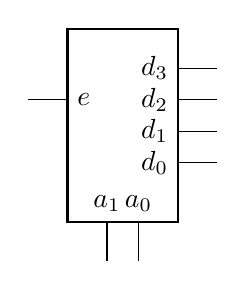
\begin{tikzpicture}
\pgfmathsetmacro{\kpin}{0.5}
\pgfmathsetmacro{\kpsep}{0.40}
\pgfmathsetmacro{\kul}{0.50}
\pgfmathsetmacro{\kxdim}{2*\kul+1*\kpsep}
\pgfmathsetmacro{\kydim}{2.5*\kul+3*\kpsep}
\draw[thick](0,0) rectangle ++(\kxdim,\kydim);
\foreach \y/\a in {2/{x}}{\draw(0,1.5*\kul+\y*\kpsep)node[right]{$e$}--++(-\kpin,0);}
\foreach \y in {0,1,2,3}{\draw(\kxdim,1.5*\kul+\y*\kpsep)node[left]{$d_{\y}$}--++(\kpin,0);}
\draw(\kxdim-\kul-0*\kpsep,0)node[above]{$a_0$}--++(0,-\kpin);
\draw(\kxdim-\kul-1*\kpsep,0)node[above]{$a_1$}--++(0,-\kpin);
\end{tikzpicture}
\end{subfigure}
\caption{ایک سے چار \عددی{(1\times 4)} خارجی منتخب کار}
\label{جدول_ترکیبی_ترتیب_نو_خارجی_منتخب_کار}
\end{figure}



\جزوحصہ{داخلی منتخب کار}
شکل \حوالہ{شکل_ترکیبی_چار_سے_ایک_داخلی_منتخب_کار_تصور} میں داخلی منتخب کار کا تصور پیش کیا گیا ہے، جہاں پیچی سوئچ کے ذریعہ \عددی{d_0} تا \عددی{d_3} میں سے ایک کا مواد مخارج منتقل کیا جا سکتا ہے۔
\begin{figure}
\centering
\begin{tikzpicture}
\pgfmathsetmacro{\kpin}{1}
\pgfmathsetmacro{\kang}{30}
\draw[thick] (0,0)node[right]{$D$}--++(-\kpin,0)--++(180-1.5*\kang:\kpin);
\foreach \a in {0,1,2,3}{\draw[thick](-\kpin,0)++(180+1.5*\kang-\a*\kang:\kpin)--++(-\kpin,0)node[left]{$d_{\a}$};}
\draw[stealth-stealth] ([shift={(180-2.25*\kang:\kpin/2)}]-\kpin,0) arc (180-2.25*\kang:180+2.25*\kang:\kpin/2);
\draw(-4.5*\kpin,-0.5)node[]{\text{\RL{داخلی مواد}}};
\draw(1.5*\kpin,-0.5)node[]{\text{\RL{خارجی مواد}}};
\end{tikzpicture}
\caption{چار سے ایک داخلی منتخب کار کا تصور۔}
\label{شکل_ترکیبی_چار_سے_ایک_داخلی_منتخب_کار_تصور}
\end{figure}

داخلی منتخب کار کو شناخت کار کی مدد سے شکل \حوالہ{شکل_ترکیبی_چار_سے_ایک_داخلی_منتخب_کار} میں حاصل کیا گیا ہے؛ شکل-ب میں اس کی علامت پیش ہے۔ یہاں مجاز و معذور صلاحیت کا شناخت کار استعمال کرکے مجاز و معذور صلاحیت کا داخلی منتخب کار حاصل کیا گیا۔ ایسا شناخت کار جس میں قابو اشارہ نہ ہو، استعمال کرتے ہوئے حاصل داخلی منتخب کار میں بھی مجاز و معذور قابو اشارہ نہیں ہو گا۔

مجاز کردہ شناخت کار \عددی{00} پتہ کی صورت میں \عددی{y_0} بلند کرے گا، جبکہ \عددی{y_1}، \عددی{y_2} اور \عددی{y_3} پست رہیں گے۔یوں دائیں تین ضرب گیٹ پست رہیں گے، جبکہ بایاں گیٹ \عددی{d_0} خارج کرے گا۔ یوں جمع گیٹ بھی \عددی{d_0} خارج کرے گا۔قابو اشارہ \عددی{e} پست کرنے سے داخلی شناخت کار معذور ہو گا اور \عددی{0} خارج کرے گا۔

تسلی کر لیں کہ مجاز حال میں ، پتہ کے دو بِٹ \عددی{a_0} اور \عددی{a_1}، چار مداخل \عددی{d_0} تا \عددی{d_1}، میں سے ایک کو منتخب کر کے خارج کرتا ہے۔
\begin{figure}
\centering
\begin{subfigure}{0.65\textwidth}
\centering
\begin{tikzpicture}
\pgfmathsetmacro{\kpin}{0.50}
\pgfmathsetmacro{\kbase}{2.5}
\pgfmathsetmacro{\kxsep}{1.25}
\pgfmathsetmacro{\kysep}{0}
\pgfmathsetmacro{\kpsep}{0.40}
\pgfmathsetmacro{\kul}{0.50}
\pgfmathsetmacro{\kxdim}{1.5}
\pgfmathsetmacro{\kydim}{2*\kul+3*\kpsep}
\pgfmathsetmacro{\kpina}{\kydim+\kysep}
\pgfmathsetmacro{\kor}{1.75}
\draw[thick](0,0) rectangle ++(\kxdim,\kydim);
\foreach \y/\a in {0/{e},2/{a_0},3/{a_1}}{\draw(0,\kul+\y*\kpsep)node[right]{$\a$}--++(-\kpin,0)node[left]{$\a$};}
\foreach \y in {0,1,2,3}{\draw(\kxdim,\kul+\y*\kpsep)node[left]{$y_{\y}$};}
\draw(\kbase+0*\kxsep,-\kysep)node[and port,scale=1,number inputs=2,rotate=-90,anchor=in 2](u0){};
\draw(\kbase+1*\kxsep,-\kysep)node[and port,scale=1,number inputs=2,rotate=-90,anchor=in 2](u1){};
\draw(\kbase+2*\kxsep,-\kysep)node[and port,scale=1,number inputs=2,rotate=-90,anchor=in 2](u2){};
\draw(\kbase+3*\kxsep,-\kysep)node[and port,scale=1,number inputs=2,rotate=-90,anchor=in 2](u3){};
\draw($(u1.out)!0.5!(u2.out)$)++(0,-\kor)node[or port,scale=1,number inputs=4,rotate=-90](u4){};
\draw(\kxdim,\kul+0*\kpsep)-|(u0.in 2);
\draw(\kxdim,\kul+1*\kpsep)-|(u1.in 2);
\draw(\kxdim,\kul+2*\kpsep)-|(u2.in 2);
\draw(\kxdim,\kul+3*\kpsep)-|(u3.in 2);
\draw(u0.out)|-(u4.in 4);
\draw(u1.out)-|(u4.in 3);
\draw(u2.out)-|(u4.in 2);
\draw(u3.out)|-(u4.in 1);
\draw(u4.out)node[below]{$D$};
\draw(u0.in 1)--++(0,\kpina)node[above]{$d_0$};
\draw(u1.in 1)--++(0,\kpina)node[above]{$d_1$};
\draw(u2.in 1)--++(0,\kpina)node[above]{$d_2$};
\draw(u3.in 1)--++(0,\kpina)node[above]{$d_3$};
\end{tikzpicture}
\caption{}
\end{subfigure}\hfill
\begin{subfigure}{0.35\textwidth}
\centering
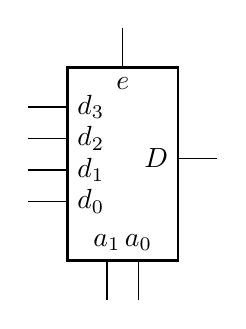
\begin{tikzpicture}
\pgfmathsetmacro{\kpin}{0.50}
\pgfmathsetmacro{\kbase}{2.5}
\pgfmathsetmacro{\kxsep}{1.25}
\pgfmathsetmacro{\kysep}{0}
\pgfmathsetmacro{\kpsep}{0.40}
\pgfmathsetmacro{\kul}{0.50}
\pgfmathsetmacro{\kxdim}{2*\kul+1*\kpsep}
\pgfmathsetmacro{\kydim}{2.5*\kul+3*\kpsep}
\pgfmathsetmacro{\kpina}{\kydim+\kysep}
\pgfmathsetmacro{\kor}{1.75}
\draw[thick](0,0) rectangle ++(\kxdim,\kydim);
\foreach \y in {0,1,2,3}{\draw(0,1.5*\kul+\y*\kpsep)node[right]{$d_{\y}$}--++(-\kpin,0);}
\foreach \y in {2}{\draw(\kxdim,\kul+\y*\kpsep)node[left]{$D$}--++(\kpin,0);}
\draw(\kxdim-\kul-0*\kpsep,0)node[above]{$a_0$}--++(0,-\kpin);
\draw(\kxdim-\kul-1*\kpsep,0)node[above]{$a_1$}--++(0,-\kpin);
\draw(\kxdim/2,\kydim)node[below]{$e$}--++(0,\kpin);
\end{tikzpicture}
\caption{}
\end{subfigure}
\caption{چار سے ایک \عددی{(4\times 1)} داخلی منتخب کار۔}
\label{شکل_ترکیبی_چار_سے_ایک_داخلی_منتخب_کار}
\end{figure}

\ابتدا{مشق}
انٹرنیٹ سے \عددی{74153} کے معلوماتی صفحات حاصل کریں۔ یہ مخلوط دور کیا کام سرانجام دیتا ہے؟
\انتہا{مشق}


\جزوحصہ{داخلی منتخب کار سے تفاعل کا حصول}
 شناخت کار کے ساتھ جمع گیٹ جوڑ کر مجموعہ ارکان ضرب کے روپ میں تفاعل کا حصول آپ دیکھ چکے۔ داخلی منتخب کار میں شناخت کار اور جمع گیٹ دونوں موجود ہیں (شکل \حوالہ{شکل_ترکیبی_چار_سے_ایک_داخلی_منتخب_کار} دیکھیں)۔یوں \عددی{n} پتہ بِٹ کا \عددی{2^n\times 1} داخلی منتخب کار سے \عددی{n} آزاد متغیر تفاعل حاصل کیا جا سکتا ہے۔اس عمل کو ایک مثال کی مدد سے سمجھتے ہیں۔
 
\ابتدا{مثال}\شناخت{مثال_ترکیبی_داخلی_منتخب_کار_سے_تفاعل_الف}
 درج ذیل تفاعل \عددی{8\times 1} داخلی منتخب کار سے حاصل کریں۔
 \begin{align*}
 F(x,y,z)=\sum (m_3,m_4,m_6,m_7)
 \end{align*}

\ترچھا{حل:}\quad
اس تفاعل کا جدول شکل \حوالہ{شکل_ترکیبی_داخلی_منتخب_کار_سے_تفاعل_الف} میں پیش ہے۔
\begin{figure}
\centering
\begin{subfigure}{0.40\textwidth}
\centering
\begin{otherlanguage}{english}
\begin{tabular}{CCC|CC}
\toprule
x&y&z&F&m\\
\midrule
0&0&0&0&m_0\\
0&0&1&0&m_1\\
0&1&0&0&m_2\\
0&1&1&1&m_3\\
1&0&0&1&m_4\\
1&0&1&0&m_5\\
1&1&0&1&m_6\\
1&1&1&1&m_7\\
\bottomrule
\end{tabular}
\end{otherlanguage}
\end{subfigure}\hfill
\begin{subfigure}{0.60\textwidth}
\centering
\begin{tikzpicture}
\pgfmathsetmacro{\kpin}{0.50}
\pgfmathsetmacro{\kpina}{0.75}
\pgfmathsetmacro{\kbase}{2.5}
\pgfmathsetmacro{\kxsep}{1.25}
\pgfmathsetmacro{\kysep}{0}
\pgfmathsetmacro{\kpsep}{0.40}
\pgfmathsetmacro{\kul}{0.50}
\pgfmathsetmacro{\kxdim}{2*\kul+2*\kpsep}
\pgfmathsetmacro{\kydim}{2.5*\kul+7*\kpsep}
\pgfmathsetmacro{\kor}{1.75}
\draw[thick](0,0) rectangle ++(\kxdim,\kydim);
\foreach \y in {0,1,2,5}{\draw(0,1.5*\kul+\y*\kpsep)node[right]{$d_{\y}$}--++(-\kpin,0);}
\foreach \y in {3,4,6,7}{\draw(0,1.5*\kul+\y*\kpsep)node[right]{$d_{\y}$}--++(-\kpina,0);}
\foreach \y in {6}{\draw(\kxdim,1.5*\kul+\y*\kpsep)node[left]{$D$}--++(\kpin,0)node[right]{$F=\sum(m_3,m_4,m_6,m_7)$};}
\draw(\kxdim-\kul-0*\kpsep,0)node[above]{$a_0$}--++(0,-\kpin)node[below]{$z$};
\draw(\kxdim-\kul-1*\kpsep,0)node[above]{$a_1$}--++(0,-\kpin)node[below]{$y$};
\draw(\kxdim-\kul-2*\kpsep,0)node[above]{$a_2$}--++(0,-\kpin)node[below]{$x$};
\draw(\kxdim/2,\kydim)node[below]{$e$}--++(0,\kpin)node[left]{$1$};
\draw(-\kpin,1.5*\kul+5*\kpsep)--(-\kpin,1.5*\kul+0*\kpsep)--++(-\kpina,0)node[left]{$0$};
\draw(-\kpina,1.5*\kul+3*\kpsep)--(-\kpina,1.5*\kul+7*\kpsep)--++(-\kpin,0)node[left]{$1$};
\draw(\kxdim-1.5*\kul,1.5*\kul+3.5*\kpsep)node[rotate=90]{\RL{داخلی منتخب کار}};
\end{tikzpicture}
\end{subfigure}
\caption{داخلی منتخب کار سے تفاعل کا حصول (برائے مثال \حوالہ{مثال_ترکیبی_داخلی_منتخب_کار_سے_تفاعل_الف})}
\label{شکل_ترکیبی_داخلی_منتخب_کار_سے_تفاعل_الف}
\end{figure}
 تفاعل کے تین آزاد متغیرات \عددی{xyz} کو \عددی{8\times 1} داخلی منتخب کار کے تین پتہ بِٹ تصور کر کے، داخلی منتخب کار کے آٹھ مداخل \عددی{d_0} تا \عددی{d_7} میں سے \عددی{d_3}، \عددی{d_4}، \عددی{d_6}، اور \عددی{d_7} کو بلند، جبکہ باقی کو پست رکھ کر تفاعل حاصل ہو گا، جو شکل \حوالہ{شکل_ترکیبی_داخلی_منتخب_کار_سے_تفاعل_الف} میں پیش ہے۔داخلی منتخب کار کو مجاز \عددی{(e=1)} رکھا گیا ہے۔

یوں پتہ \عددی{000}، \عددی{001}، \عددی{010}،اور \عددی{101} کی صورت میں داخلی منتخب کار بالترتیب \عددی{d_0}، \عددی{d_1}، \عددی{d_2}، اور \عددی{d_5} پر فراہم مواد خارج کرے گا؛ ان تمام کو پست رکھ کر درکار تفاعل کی پست صورت حاصل ہو گی۔اسی طرح پتہ \عددی{011}، \عددی{100}، \عددی{110}، اور \عددی{11} کی صورت میں بالترتیب \عددی{d_3}، \عددی{d_4}، \عددی{d_6}، اور \عددی{d_7} کے مواد خارج ہوں گے؛انہیں بلند رکھ کر تفاعل کی بلند صورت حاصل ہو گی۔کسی ایک لمحہ پر پتہ صرف ایک قیمت رکھ سکتا ہے۔
\انتہا{مثال}

 \عددی{n} آزاد متغیر تفاعل ، \عددی{(n-1)}پتہ بِٹ کے داخلی منتخب کار سے بھی حاصل کیا جا سکتا ہے۔یہاں کوئی بھی \عددی{(n-1)} متغیرات بطور داخلی منتخب کار کے پتہ استعمال ہوں گے، جبکہ ایک متغیر بطور مداخل استعمال ہو گا۔ ایک مثال کی مدد سے ایسا کرنا سیکھتے ہیں۔


\ابتدا{مثال}\شناخت{مثال_ترکیبی_داخلی_منتخب_کار_سے_تفاعل_ب}
 درج بالا مثال میں دیا گیا تفاعل \عددی{ F(x,y,z)=\sum (m_3,m_4,m_6,m_7)} دو پتہ بِٹ کے \عددی{4\times 1} داخلی منتخب کار سے حاصل کریں۔

\ترچھا{حل:}\quad
شکل \حوالہ{شکل_ترکیبی_داخلی_منتخب_کار_سے_تفاعل_ب} میں تفاعل کا جدول ایک نئے انداز میں لکھا گیا ہے۔
\begin{figure}
\centering
\begin{subfigure}{0.40\textwidth}
\centering
\begin{otherlanguage}{english}
\begin{tabular}{CC|CCC}
\toprule
x&y&z&F&\\
\midrule
0&0&0&0&\multirow{2}{*}{$F=0$}\\
0&0&1&0&\\
\midrule
0&1&0&0&\multirow{2}{*}{$F=z$}\\
0&1&1&1&\\
\midrule
1&0&0&1&\multirow{2}{*}{$F=\overline{z}$}\\
1&0&1&0&\\
\midrule
1&1&0&1&\multirow{2}{*}{$F=1$}\\
1&1&1&1&\\
\bottomrule
\end{tabular}
\end{otherlanguage}
\end{subfigure}\hfill
\begin{subfigure}{0.60\textwidth}
\centering
\begin{tikzpicture}
\pgfmathsetmacro{\kpin}{0.50}
\pgfmathsetmacro{\kpina}{2}
\pgfmathsetmacro{\kbase}{2.5}
\pgfmathsetmacro{\kxsep}{1.25}
\pgfmathsetmacro{\kysep}{0}
\pgfmathsetmacro{\kpsep}{0.40}
%\pgfmathsetmacro{\kpsepa}{1.2}
\pgfmathsetmacro{\kul}{0.50}
\pgfmathsetmacro{\kxdim}{2*\kul+2*\kpsep}
\pgfmathsetmacro{\kydim}{2.5*\kul+5*\kpsep}
\pgfmathsetmacro{\kor}{1.75}
\draw[thick](0,0) rectangle ++(\kxdim,\kydim);
\foreach \y/\d in {0/0,1/1,3/2,5/3}{\draw(0,1.5*\kul+\y*\kpsep)node[right]{$d_{\d}$};}
%\foreach \y in {3,4,6,7}{\draw(0,1.5*\kul+\y*\kpsep)node[right]{$d_{\y}$}--++(-\kpina,0);}
\foreach \y in {2}{\draw(\kxdim,1.5*\kul+\y*\kpsep)node[left]{$D$}--++(\kpin,0)node[right]{$F(x,y,z)$};}
\draw(\kxdim-\kul-0*\kpsep,0)node[above]{$a_0$}--++(0,-\kpin)node[below]{$y$};
\draw(\kxdim-\kul-1*\kpsep,0)node[above]{$a_1$}--++(0,-\kpin)node[below]{$x$};
%\draw(\kxdim-\kul-2*\kpsep,0)node[above]{$a_2$}--++(0,-\kpin)node[below]{$x$};
%\draw(\kxdim/2,\kydim)node[below]{$e$}--++(0,\kpin)node[left]{$1$};
\draw(\kxdim-1.5*\kul,1.5*\kul+3*\kpsep)node[rotate=90]{\RL{داخلی منتخب کار}};
\draw(0,1.5*\kul+3*\kpsep)node[not port,scale=1,anchor=out](u1){};
\draw(u1.in)--++(-\kpin,0)node[left]{$z$}coordinate(aaa)++(0,\kpin)coordinate(bbb);
\draw(0,1.5*\kul+0*\kpsep)--($(aaa)!(0,1.5*\kul+0*\kpsep)!(bbb)$)node[left]{$0$};
\draw(0,1.5*\kul+5*\kpsep)--($(aaa)!(0,1.5*\kul+5*\kpsep)!(bbb)$)node[left]{$1$};
\draw(0,1.5*\kul+1*\kpsep)-|(u1.in);
\end{tikzpicture}
\end{subfigure}
\caption{داخلی منتخب کار سے تفاعل کا حصول (برائے مثال \حوالہ{مثال_ترکیبی_داخلی_منتخب_کار_سے_تفاعل_ب})}
\label{شکل_ترکیبی_داخلی_منتخب_کار_سے_تفاعل_ب}
\end{figure}
 آزاد متغیرات \عددی{xy} کے دائیں کھڑی لکیر کھینچ گئی، اور \عددی{xy} کی قیمت کے مطابق جدول کے چار حصے کیے گئے ۔پہلے (بالائی) حصہ میں (جہاں \عددی{xy=00}ہے) تفاعل \عددی{F} کی قیمت بدستور \عددی{0} ہے، لہٰذا اس حصہ کے اضافی قطار میں \عددی{F=0} لکھا گیا۔ دوسرے حصے ( \عددی{xy=01}) کی دونوں صفوں میں \عددی{z} کی قیمت اور تفاعل \عددی{F} کی قیمت برابر ہیں، لہٰذا یہاں \عددی{F=z} لکھا گیا۔ تیسرے حصے (\عددی{xy=10}) میں \عددی{z} اور \عددی{F} کی قیمتیں آپ میں متمم ہیں، لہٰذا یہاں \عددی{F=\overline{z}} لکھا گیا ہے۔آخری حصہ ( \عددی{xy=11}) میں تفاعل بدستور بلند ہے، لہٰذا یہاں \عددی{F=1} لکھا گیا۔


شکل \حوالہ{شکل_ترکیبی_داخلی_منتخب_کار_سے_تفاعل_ب} میں اس جدول سے حاصل دور دکھایا گیا ہے، جہاں (مجاز و معذور صلاحیت نہ رکھنے والا) \عددی{4\times 1} داخلی منتخب کار استعمال کیا گیا۔پتہ \عددی{xy=00} کی صورت میں داخلی منتخب کار مداخل \عددی{d_0} کا مواد خارج کرے گا۔یوں \عددی{d_0} پر \عددی{0} مہیا کر کے اس صورت میں تفاعل کی درست قیمت حاصل کی گئی۔اسی طرح \عددی{xy=01} کی صورت میں \عددی{d_1} کا مواد خارج کیا جائے گا، لہٰذا یہاں متغیر \عددی{z} فراہم کر کے تفاعل کی درست قیمت حاصل کی گئی۔اسی طرح \عددی{xy=10} کی صورت میں \عددی{d_2} کا مواد مخارج کیا جائے گا، لہٰذا یہاں \عددی{\overline{z}} فراہم کر کے تفاعل کی درست قیمت حاصل کی گئی، اور آخر میں \عددی{xy=11} کی صورت میں تفاعل بدستور بلند رہتا ہے، لہٰذا \عددی{d_3} پر \عددی{1} مہیا کیا گیا۔
\انتہا{مثال}


\حصہ{متوازی ثنائی ضرب کار}
حسابی اعمال میں ضرب کا کردار کلیدی ہے۔ثنائی اعداد کی ضرب کا عمل بالکل اعشاری اعداد کی ضرب کی طرح ہے۔دو بِٹ ثنائی اعداد \عددی{a} اور \عددی{b} کی ضرب درج ذیل ہے، جہاں ان ثنائی اعداد کو \عددی{a_1a_0} اور \عددی{b_1b_0} لکھا گیا ہے ۔

\begin{align*}
\begin{array}{cccc}
&& b_1&b_0\\
&& a_1&a_0\\
\cline{3-4}
&& a_0b_1&a_0b_0\\
&a_1b_1&a_1b_0&\\
\cline{1-4}
p_3&p_2&p_1&p_0
\end{array}
\end{align*}
یہاں درج ذیل ہوں گے، جنہیں ثنائی جمع کار کی مساوات \حوالہ{مساوات_ترکیبی_نصف_جمع_کار} کی مدد سے حاصل کیا گیا، اور جن سے شکل \حوالہ{شکل_ترکیبی_ثنائی_متوازی_دو_ضرب_کار} میں پیش، دو بِٹ متوازی ثنائی ضرب کار حاصل ہو گا۔
\begin{align*}
p_0&=a_0b_0\\
p_1&=(a_1b_0)\oplus(a_0b_1)\\
p_2&=(a_1b_1)\oplus(a_1b_0a_0b_1)\\
p_3&=a_1b_1a_1b_0a_0b_1=a_1a_0b_1b_0
\end{align*}


\begin{figure}
\centering
\begin{tikzpicture}
\pgfmathsetmacro{\kxstep}{2}
\pgfmathsetmacro{\kystep}{2}
\pgfmathsetmacro{\kystepa}{2.5}
\pgfmathsetmacro{\ksh}{0.4}
\pgfmathsetmacro{\ksha}{1.25}
\draw(0,3.5*\kystep)node[and port,scale=1,number inputs=2,anchor=out](u0){u0} (u0.out)node[right]{$p_0$};
\draw(0,2.5*\kystep)node[xor port,scale=1,number inputs=2,anchor=out](u1){u1}(u1.out)node[right]{$p_1$};
\draw(0,1*\kystep)node[xor port,scale=1,number inputs=2,anchor=out](u2){u2}(u2.out)node[right]{$p_2$};
\draw(0,0*\kystep)node[and port,scale=1,number inputs=4,anchor=out](u3){u3}(u3.out)node[right]{$p_3$};
\draw(u1.in 1)--++(0,\ksh)--++(-\kxstep,0)node[and port,scale=1,number inputs=2,anchor=out](u4){u4}
 (u4.in 1)node[left]{$a_1$} (u4.in 2)node[left]{$b_0$};
\draw(u1.in 2)--++(0,-\ksh)--++(-\kxstep,0)node[and port,scale=1,number inputs=2,anchor=out](u5){u5}
 (u5.in 1)node[left]{$a_0$} (u5.in 2)node[left]{$b_1$};
\draw(u0.in 1)--($(u4.in 1)!(u0.in 1)!(u4.in 2)$)node[left]{$a_0$};
\draw(u0.in 2)--($(u4.in 1)!(u0.in 2)!(u4.in 2)$)node[left]{$b_0$};
\draw(u2.in 1)--++(0,\ksh)--++(-\kxstep,0)node[and port,scale=1,number inputs=2,anchor=out](u6){u6}
 (u6.in 1)node[left]{$a_1$} (u6.in 2)node[left]{$b_1$};
\draw(u2.in 2)--++(0,-\ksh)--++(-\kxstep,0)node[and port,scale=1,number inputs=4,anchor=out](u7){u7}
 (u7.in 1)node[left]{$a_0$} (u7.in 2)node[left]{$a_1$} (u7.in 3)node[left]{$b_0$} (u7.in 4)node[left]{$b_1$};
 \draw(u3.in 1)--($(u4.in 1)!(u3.in 1)!(u4.in 2)$)node[left]{$a_0$}(u3.in 2)--($(u4.in 1)!(u3.in 2)!(u4.in 2)$)node[left]{$a_1$}(u3.in 3)--($(u4.in 1)!(u3.in 3)!(u4.in 2)$)node[left]{$b_0$} (u3.in 4)--($(u4.in 1)!(u3.in 4)!(u4.in 2)$)node[left]{$b_1$};
\end{tikzpicture}
\caption{دو بِٹ ثنائی متوازی ضرب کار}
\label{شکل_ترکیبی_ثنائی_متوازی_دو_ضرب_کار}
\end{figure}


 اگرچہ زیادہ بِٹ ضرب کار اس طریقہ کار سے تشکیل دیے جا سکتے ہیں؛ بد قسمتی سے، اعداد کے بِٹ کی تعداد بڑھانے سے ضرب کار میں درکار گیٹوں کی تعداد بہت تیزی سے بڑھتی ہے (محض آٹھ یا سولہ بِٹ ضرب کار میں بھی مستعمل گیٹوں کی تعداد بہت زیادہ ہو گی)، لہٰذا ایسا کرنا مہنگا ثابت ہو گا۔ عموماً زیادہ بِٹ کے ضرب کار مکمل جمع کار کی مدد سے حاصل کیے جاتے ہیں۔ اس طریقہ کو تین بِٹ ثنائی اعداد کی ضرب کو مثال بنا کر سیکھتے ہیں۔

تین بِٹ اعداد \عددی{b_2b_1b_0} اور \عددی{a_2a_1a_0} کی ضرب درج ذیل ہے، جس سے شکل \حوالہ{شکل_ترکیبی_تین_بٹ_ضرب_کار} میں پیش تین بِٹ ثنائی ضرب کار حاصل ہو گا۔ اس طریقہ کار سے با آسانی زیادہ بِٹ کے ثنائی ضرب کار بنائے جا سکتے ہیں۔
\begin{gather}
\begin{aligned}\label{مساوات_ترکیبی_تین_بٹ_ضرب_کار}
\begin{array}{cccccc}
&&&b_2& b_1&b_0\\
&&&a_2& a_1&a_0\\
\cline{4-6}
&&&a_0b_2& a_0b_1&a_0b_0\\
&&a_1b_2&a_1b_1&a_1b_0&\\
&a_2b_2&a_2b_1&a_2b_0&\\
\cline{1-6}
p_5&p_4&p_3&p_2&p_1&p_0
\end{array}
\end{aligned}
\end{gather}
%
\begin{figure}
\centering
\begin{tikzpicture}
\pgfmathsetmacro{\kxa}{3.5}
\pgfmathsetmacro{\kya}{1.25}
\draw(0*\kxa,2*\kya)node[and port,scale=1,number inputs=2](u2){u2};
\draw(0*\kxa,1*\kya)node[and port,scale=1,number inputs=2](u1){u1};
\draw(0*\kxa,0*\kya)node[and port,scale=1,number inputs=2](u0){u0};
\draw(1*\kxa,2*\kya)node[and port,scale=1,number inputs=2](u5){u5};
\draw(1*\kxa,1*\kya)node[and port,scale=1,number inputs=2](u4){u4};
\draw(1*\kxa,0*\kya)node[and port,scale=1,number inputs=2](u3){u3};
\draw(2*\kxa,2*\kya)node[and port,scale=1,number inputs=2](u8){u8};
\draw(2*\kxa,1*\kya)node[and port,scale=1,number inputs=2](u7){u7};
\draw(2*\kxa,0*\kya)node[and port,scale=1,number inputs=2](u6){u6};
\draw(u0.in 1)node[left]{$a_0$} (u0.in 2)node[left]{$b_2$} (u0.out)node[right]{$A_2$};
\draw(u1.in 1)node[left]{$a_0$} (u1.in 2)node[left]{$b_1$} (u1.out)node[right]{$A_1$};
\draw(u2.in 1)node[left]{$a_0$} (u2.in 2)node[left]{$b_0$} (u2.out)node[right]{$A_0$};
\draw(u3.in 1)node[left]{$a_1$} (u3.in 2)node[left]{$b_2$} (u3.out)node[right]{$B_2$};
\draw(u4.in 1)node[left]{$a_1$} (u4.in 2)node[left]{$b_1$} (u4.out)node[right]{$B_1$};
\draw(u5.in 1)node[left]{$a_1$} (u5.in 2)node[left]{$b_0$} (u5.out)node[right]{$B_0$};
\draw(u6.in 1)node[left]{$a_2$} (u6.in 2)node[left]{$b_2$} (u6.out)node[right]{$C_2$};
\draw(u7.in 1)node[left]{$a_2$} (u7.in 2)node[left]{$b_1$} (u7.out)node[right]{$C_1$};
\draw(u8.in 1)node[left]{$a_2$} (u8.in 2)node[left]{$b_0$} (u8.out)node[right]{$C_0$};
\end{tikzpicture}\vspace{1cm}
\begin{tikzpicture}
\pgfmathsetmacro{\kpin}{0.50}
\pgfmathsetmacro{\kul}{0.5}
\pgfmathsetmacro{\kxbase}{1.5}
\pgfmathsetmacro{\kysep}{2.25}
\pgfmathsetmacro{\kxdim}{1.5}
\pgfmathsetmacro{\kydim}{1}
\pgfmathsetmacro{\kxsep}{\kxbase+\kxdim-2*\kul}
\draw[thick](0,0)node[below right]{$u_9$} rectangle ++(\kxdim,\kydim);
\draw[thick](\kxsep,0)node[below right]{$u_{10}$} rectangle ++(\kxdim,\kydim);
\draw[thick](2*\kxsep,0)node[below right]{$u_{11}$} rectangle ++(\kxdim,\kydim);
\draw[thick](\kxbase,\kysep)node[below right]{$u_{12}$} rectangle ++(\kxdim,\kydim);
\draw[thick](\kxbase+\kxsep,\kysep)node[below right]{$u_{13}$} rectangle ++(\kxdim,\kydim);
\draw[thick](\kxbase+2*\kxsep,\kysep)node[below right]{$u_{14}$} rectangle ++(\kxdim,\kydim);
\draw(\kul,\kydim)node[below]{$z$}--++(0,\kpin)node[above]{$C_2$};
\draw(\kxsep+\kxdim-\kul,\kydim)node[below]{$y$}--++(0,\kpin)node[above]{$C_1$};
\draw(2*\kxsep+\kxdim-\kul,\kydim)node[below]{$y$}--++(0,\kpin)node[above]{$C_0$};
\draw(0,\kydim/2)node[right]{$c_{\text{خ}}$}--++(-\kpin,0)--++(0,-\kydim/2-\kpin)node[below]{$p_5$};
\draw(\kxdim-\kul,0)node[above]{$s$}--++(0,-\kpin)node[below]{$p_4$};
\draw(\kxsep+\kxdim-\kul,0)node[above]{$s$}--++(0,-\kpin)node[below]{$p_3$};
\draw(2*\kxsep+\kxdim-\kul,0)node[above]{$s$}--++(0,-\kpin)node[below]{$p_2$};
\draw(\kxdim-\kul,\kydim)node[below]{$y$}--++(0,\kysep-\kydim/2)--++(\kxbase-\kxdim+\kul,0)
node[right]{$c_{\text{خ}}$};
\draw(\kxsep+\kul,\kydim)node[below]{$z$}--++(0,\kysep-\kydim)node[above]{$s$};
\draw(2*\kxsep+\kul,\kydim)node[below]{$z$}--++(0,\kysep-\kydim)node[above]{$s$};
\draw(\kxbase+\kxdim,\kysep+\kydim/2)node[left]{$c_{\text{د}}$}--++(\kxsep-\kxdim,0)node[right]{$c_{\text{خ}}$};
\draw(\kxbase+\kxsep+\kxdim,\kysep+\kydim/2)node[left]{$c_{\text{د}}$}--++(\kxsep-\kxdim,0)
node[right]{$c_{\text{خ}}$};
\draw(\kxbase+2*\kxsep+\kxdim,\kysep+\kydim/2)node[left]{$c_{\text{د}}$}--++(\kpin/2,0)node[right]{$0$};
\draw(\kxdim,\kydim/2)node[left]{$c_{\text{د}}$}--++(\kxsep-\kxdim,0)node[right]{$c_{\text{خ}}$};
\draw(\kxsep+\kxdim,\kydim/2)node[left]{$c_{\text{د}}$}--++(\kxsep-\kxdim,0)node[right]{$c_{\text{خ}}$};
\draw(2*\kxsep+\kxdim,\kydim/2)node[left]{$c_{\text{د}}$}--++(\kpin/2,0)node[right]{$0$};
\draw(\kxbase+\kul,\kysep+\kydim)node[below]{$z$}--++(0,\kpin)node[above]{$0$};
\draw(\kxbase+\kxdim-\kul,\kysep+\kydim)node[below]{$y$}--++(0,\kpin)node[above]{$B_2$};
\draw(\kxbase+\kxsep+\kul,\kysep+\kydim)node[below]{$z$}--++(0,\kpin)node[above]{$A_2$};
\draw(\kxbase+\kxsep+\kxdim-\kul,\kysep+\kydim)node[below]{$y$}--++(0,\kpin)node[above]{$B_1$};
\draw(\kxbase+2*\kxsep+\kul,\kysep+\kydim)node[below]{$z$}--++(0,\kpin)node[above]{$A_1$};
\draw(\kxbase+2*\kxsep+\kxdim-\kul,\kysep+\kydim)node[below]{$y$}--++(0,\kpin)node[above]{$B_0$};
\draw(\kxbase+2*\kxsep+\kxdim-\kul,\kysep)node[above]{$s$}--++(0,-\kysep-\kpin)node[below]{$p_1$};
\draw(\kxbase+3*\kxsep+\kul,\kysep+\kydim+\kpin)node[above]{$A_0$}--++(0,-\kpin-\kydim-\kysep-\kpin)node[below]{$p_0$};
\end{tikzpicture}
\caption{تین بِٹ ثنائی ضرب کار }
\label{شکل_ترکیبی_تین_بٹ_ضرب_کار}
\end{figure}

اس شکل میں \عددی{9} ضرب گیٹ اور \عددی{ 6} مکمل جمع کار مستعمل ہیں۔ ضرب گیٹ \عددی{u_1} مداخل \عددی{a_0} اور \عددی{b_1} کا منطقی ضرب \عددی{A_1=a_0b_1} دے گا، جو مکمل جمع کار \عددی{u_{14}} کا \عددی{z} مداخل ہے۔ شکل میں \عددی{u_1} کے مخارج سے \عددی{u_{14}} کے \عددی{z} مداخل تک تار نظر پوش کرتے ہوئے دونوں کو ایک نام \عددی{(A_1)} سے پکارا گیا ہے۔ دو نقطوں کو ایک نام سے پکارنا، دونوں کو آپس میں تار سے جوڑنے کے مترادف ہے۔
